\section{Results}
In this section, we present the final results. Additionnally to these results,
we also provide tuning results that have guided our algorithm selection.

\subsection{F1}
Figure~\ref{fig:f1} shows the f1-scores for the six datasets.  We
observe that on the long run, the Mondrian algorithm with 5 or 10 trees achieves
the best f1-scores.  On most of the datasets (\banosdataset, \recofitdataset,
RandomTree) the best Mondrian is followed by the NaiveBayes classifiers. 

\begin{figure*}[ht]
	\begin{subfigure}[t]{.5\linewidth}
		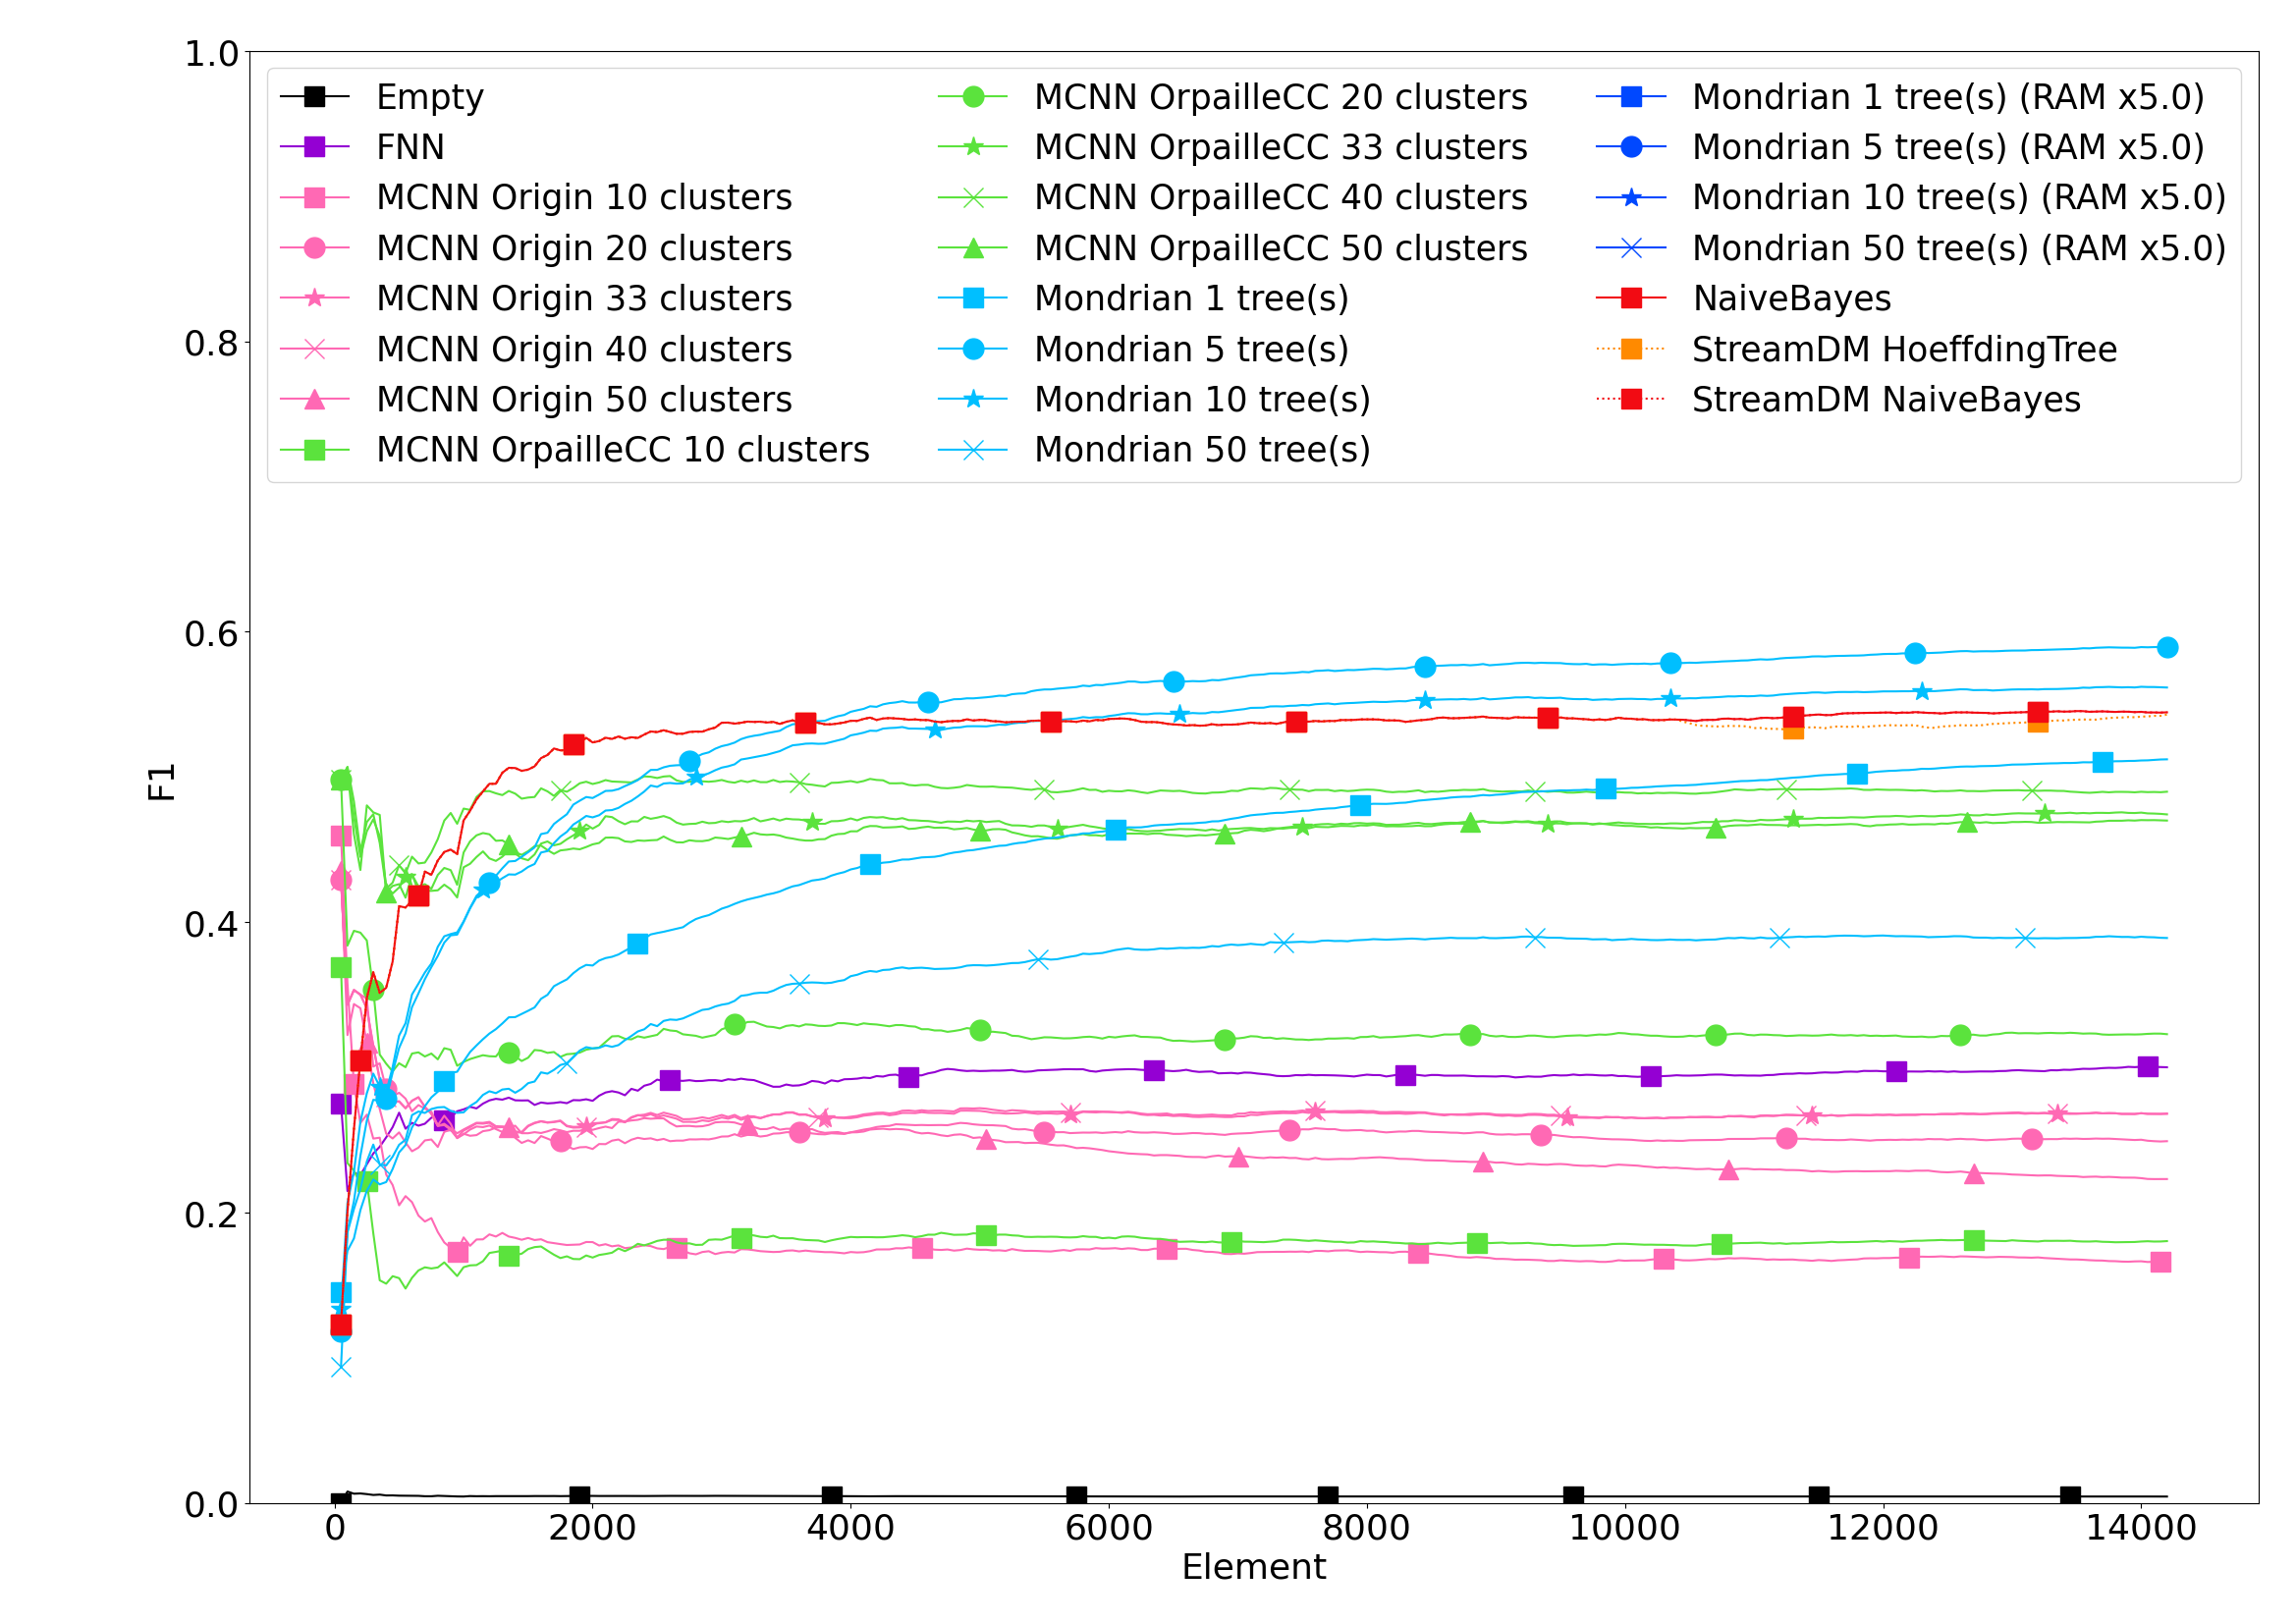
\includegraphics[width=\linewidth]{figures/results/banos_3_f1.png}
		\caption{\banosdataset}
		\label{fig:f1-banos}
	\end{subfigure}
	\begin{subfigure}[t]{.5\linewidth}
		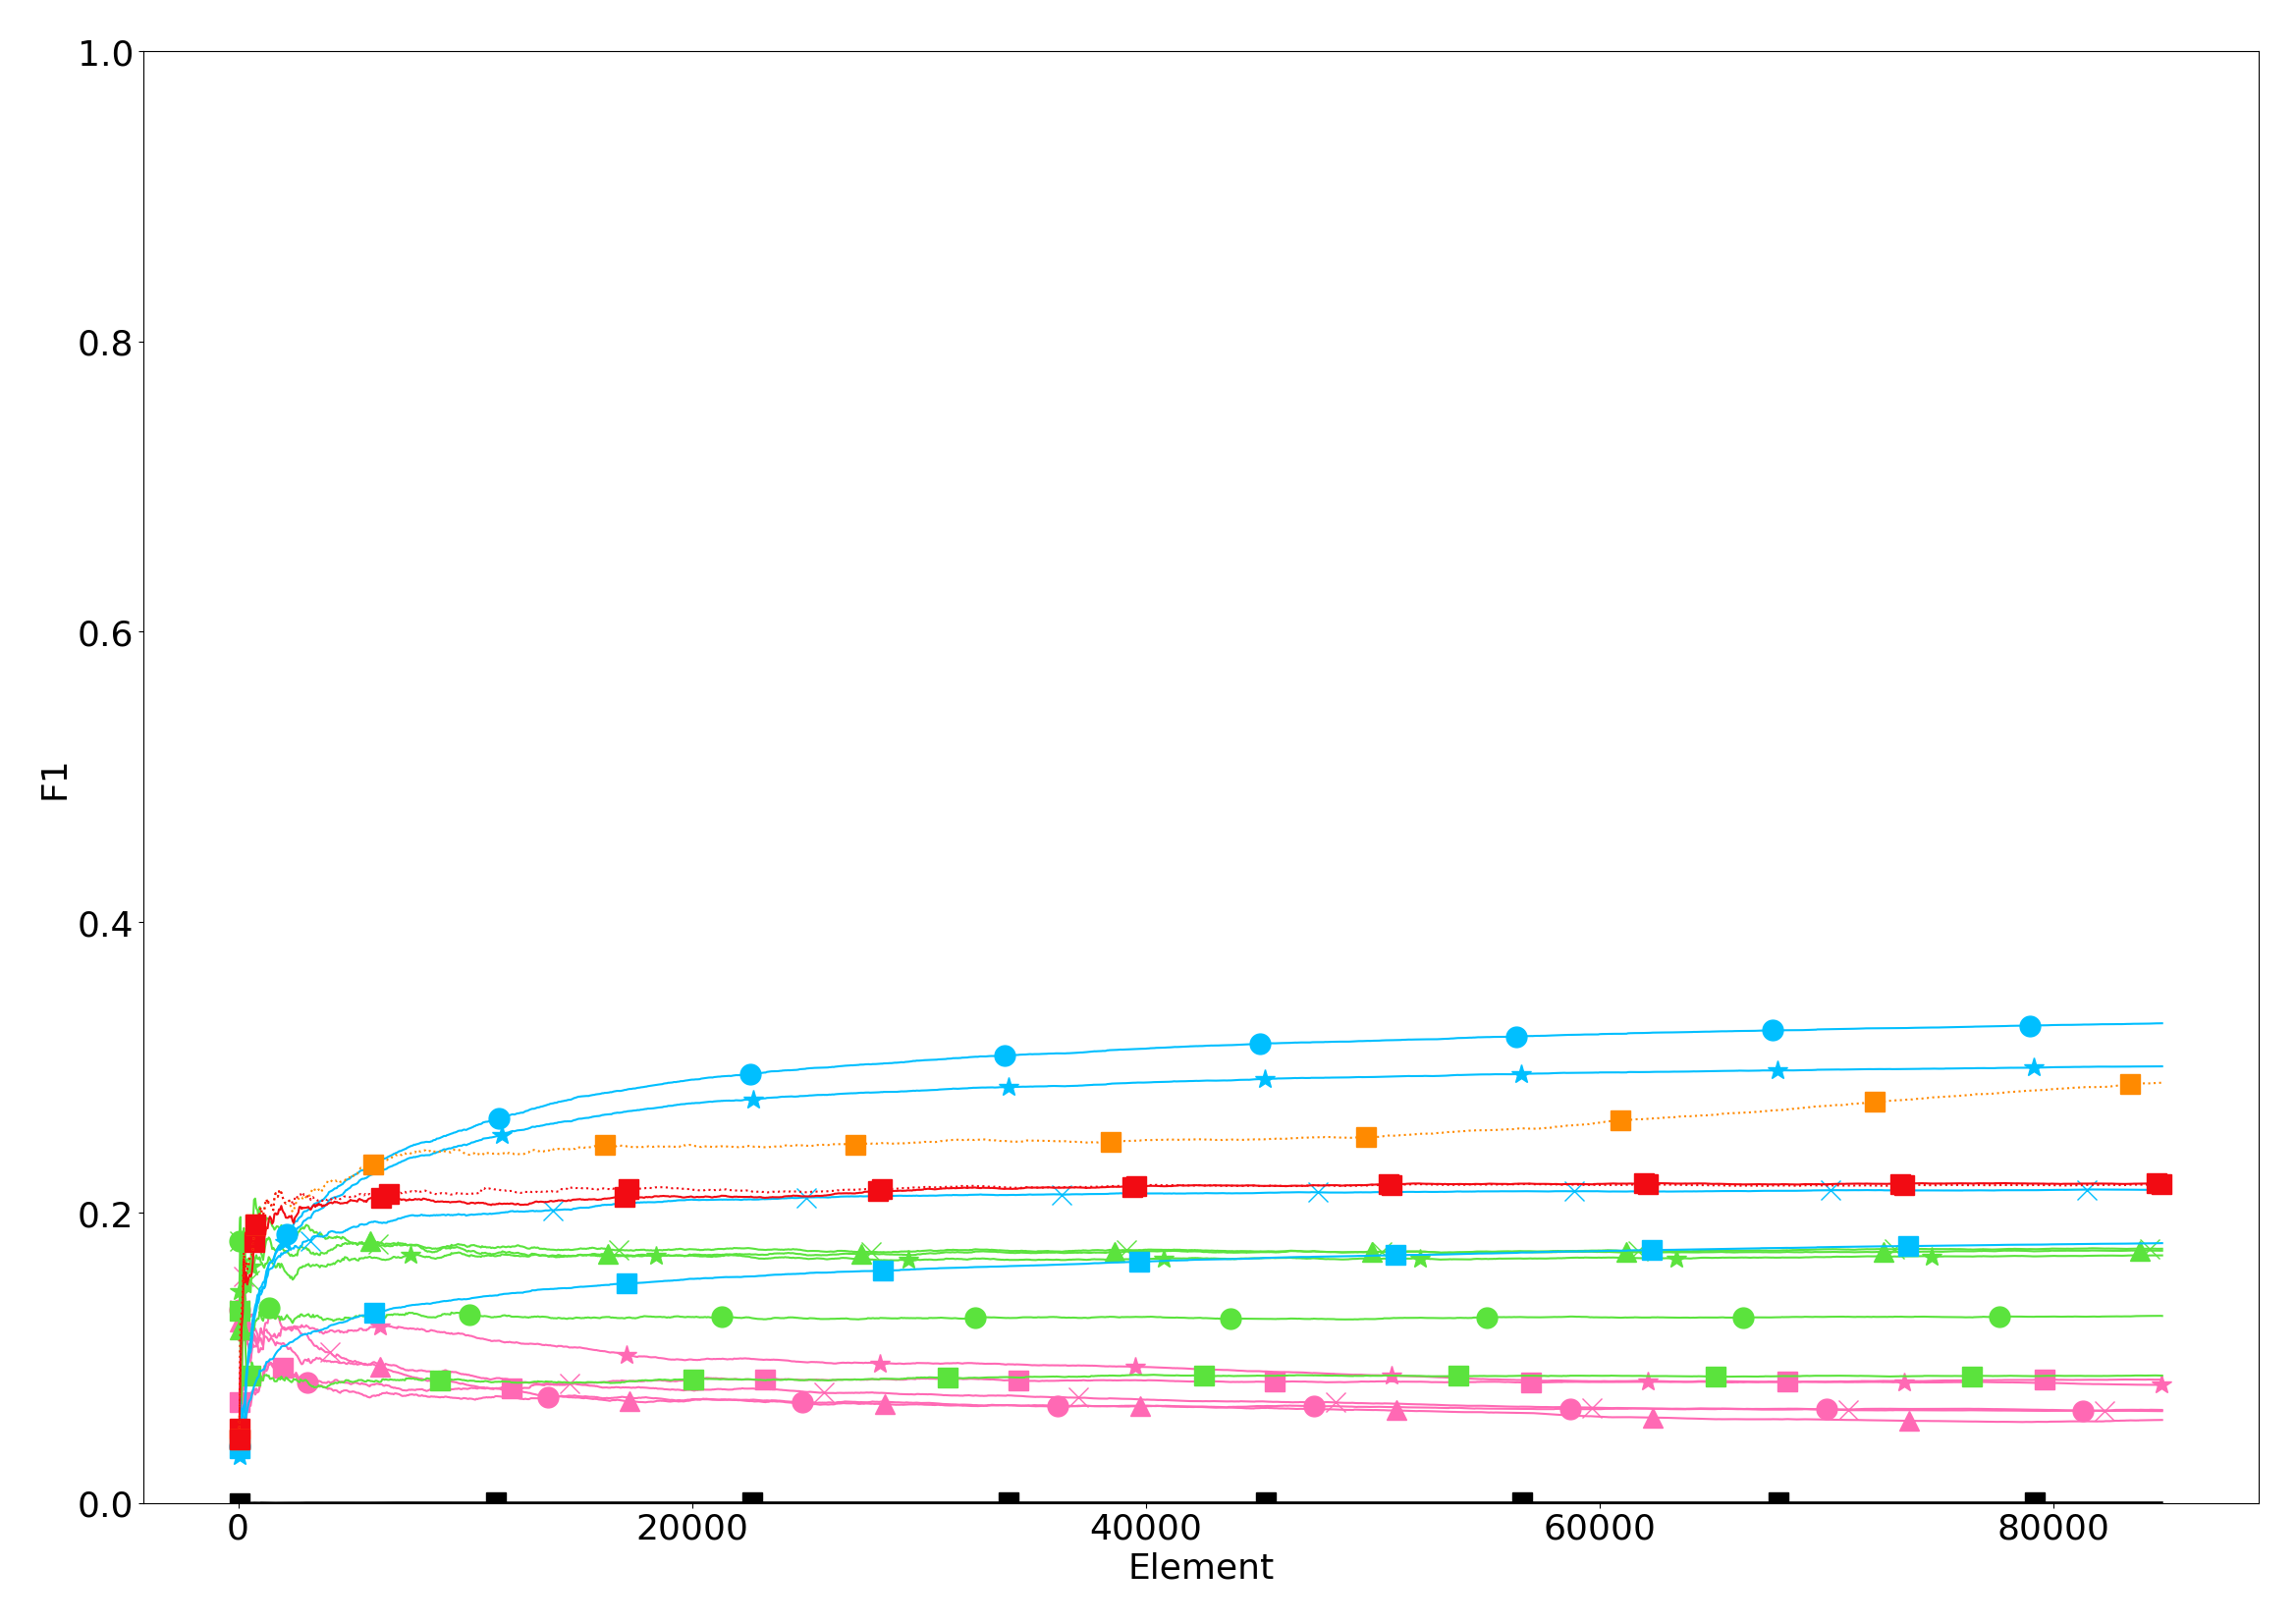
\includegraphics[width=\linewidth]{figures/results/recofit_3_f1.png}
		\caption{\recofitdataset}
		\label{fig:f1-recofit}
	\end{subfigure}
	\begin{subfigure}[t]{.5\linewidth}
		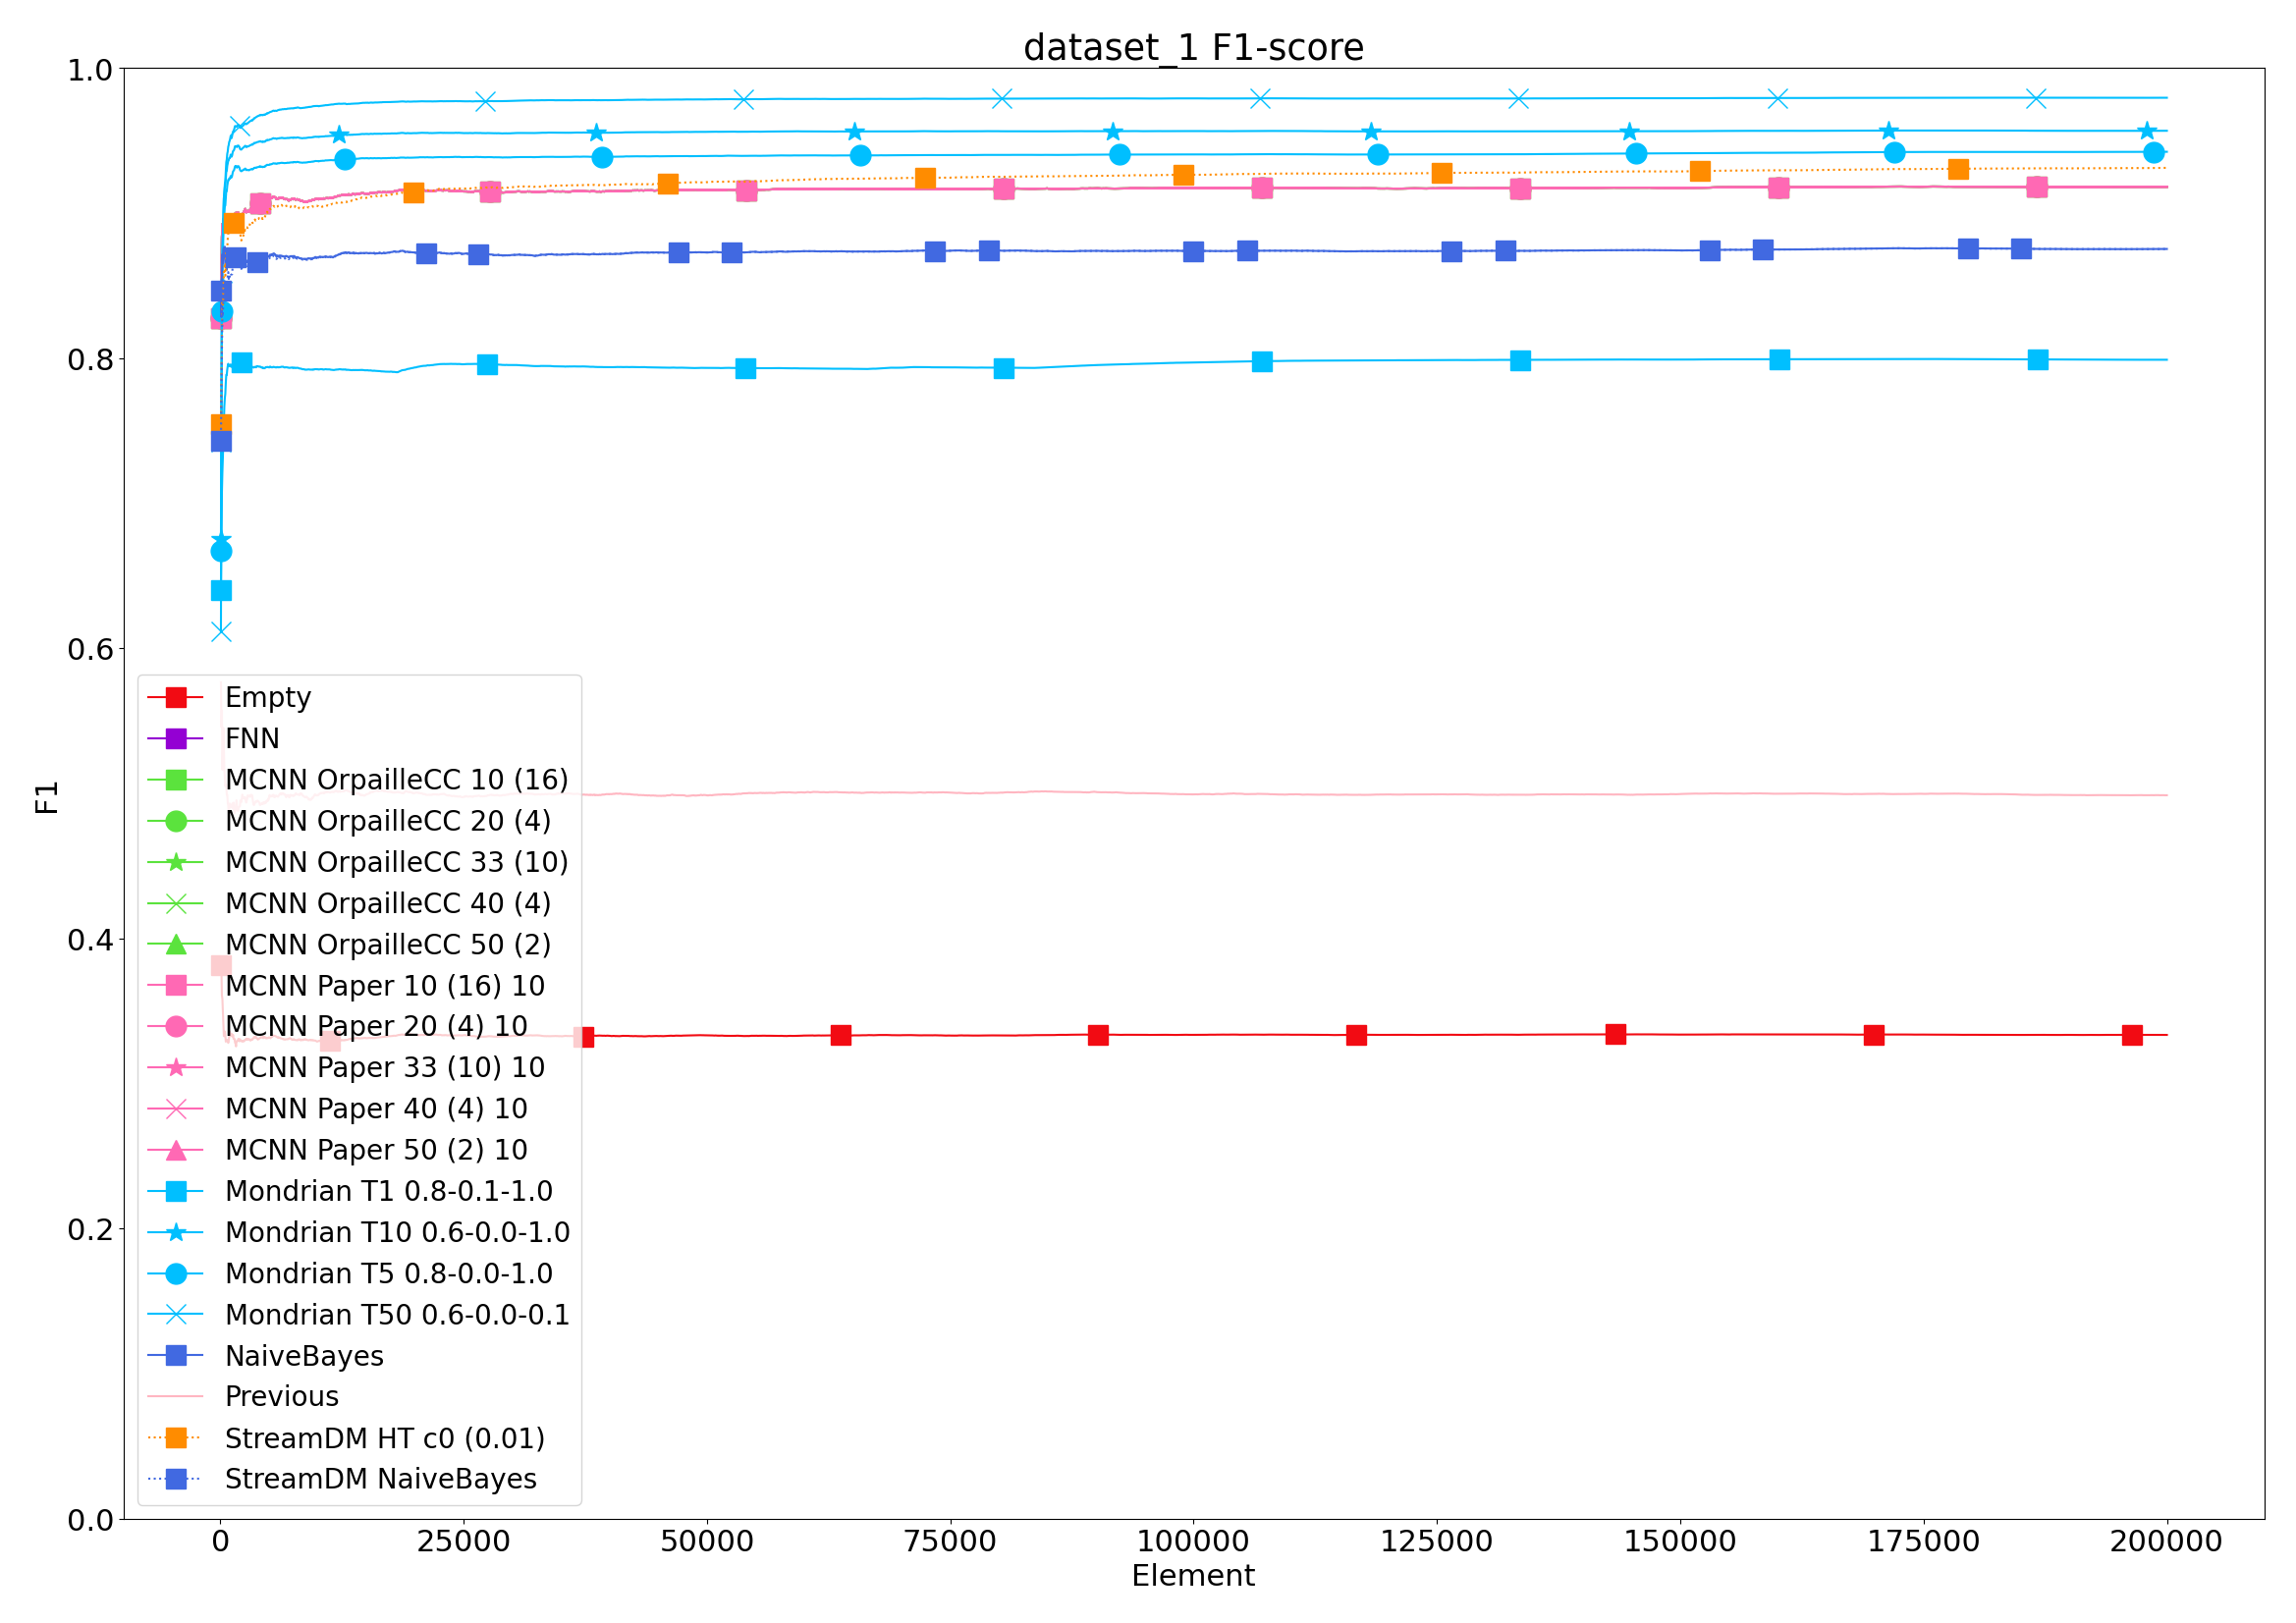
\includegraphics[width=\linewidth]{figures/results/dataset_1_f1.png}
		\caption{Hyperplane}
		\label{fig:f1-dataset_1}
	\end{subfigure}
	\begin{subfigure}[t]{.5\linewidth}
		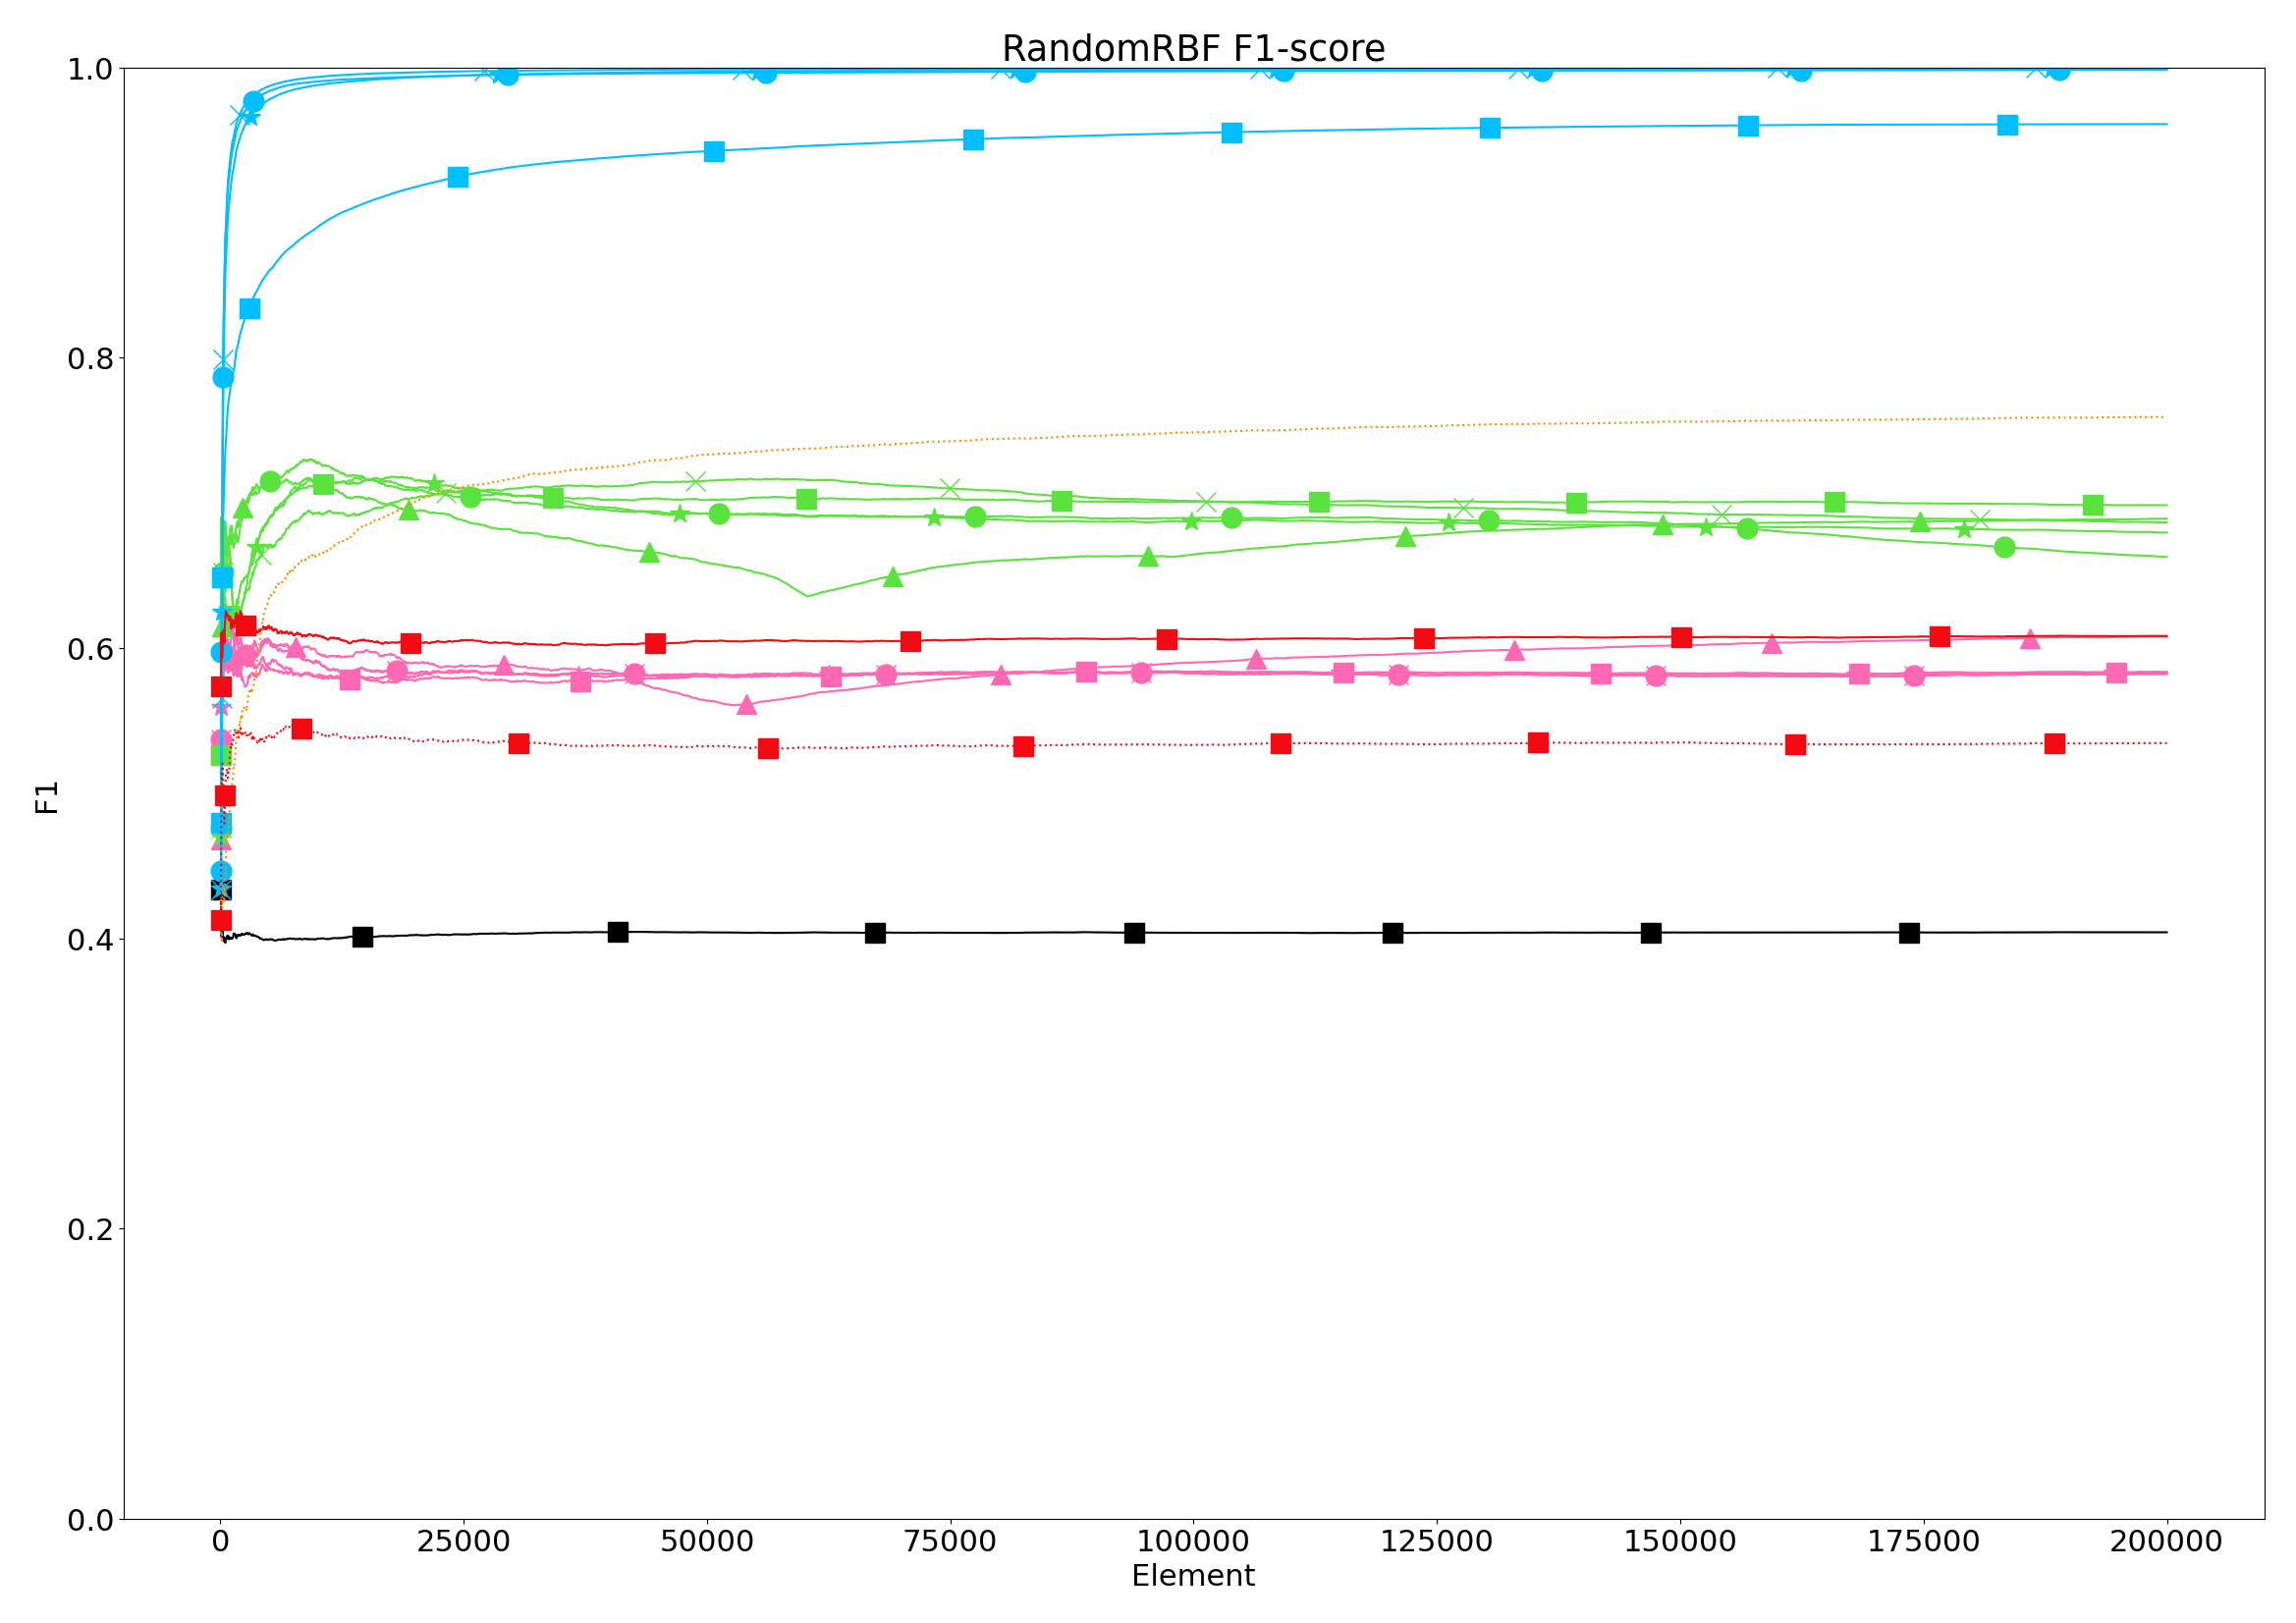
\includegraphics[width=\linewidth]{figures/results/dataset_2_f1.png}
		\caption{RandomRBF}
		\label{fig:f1-dataset_2}
	\end{subfigure}
	\begin{subfigure}[t]{.5\linewidth}
		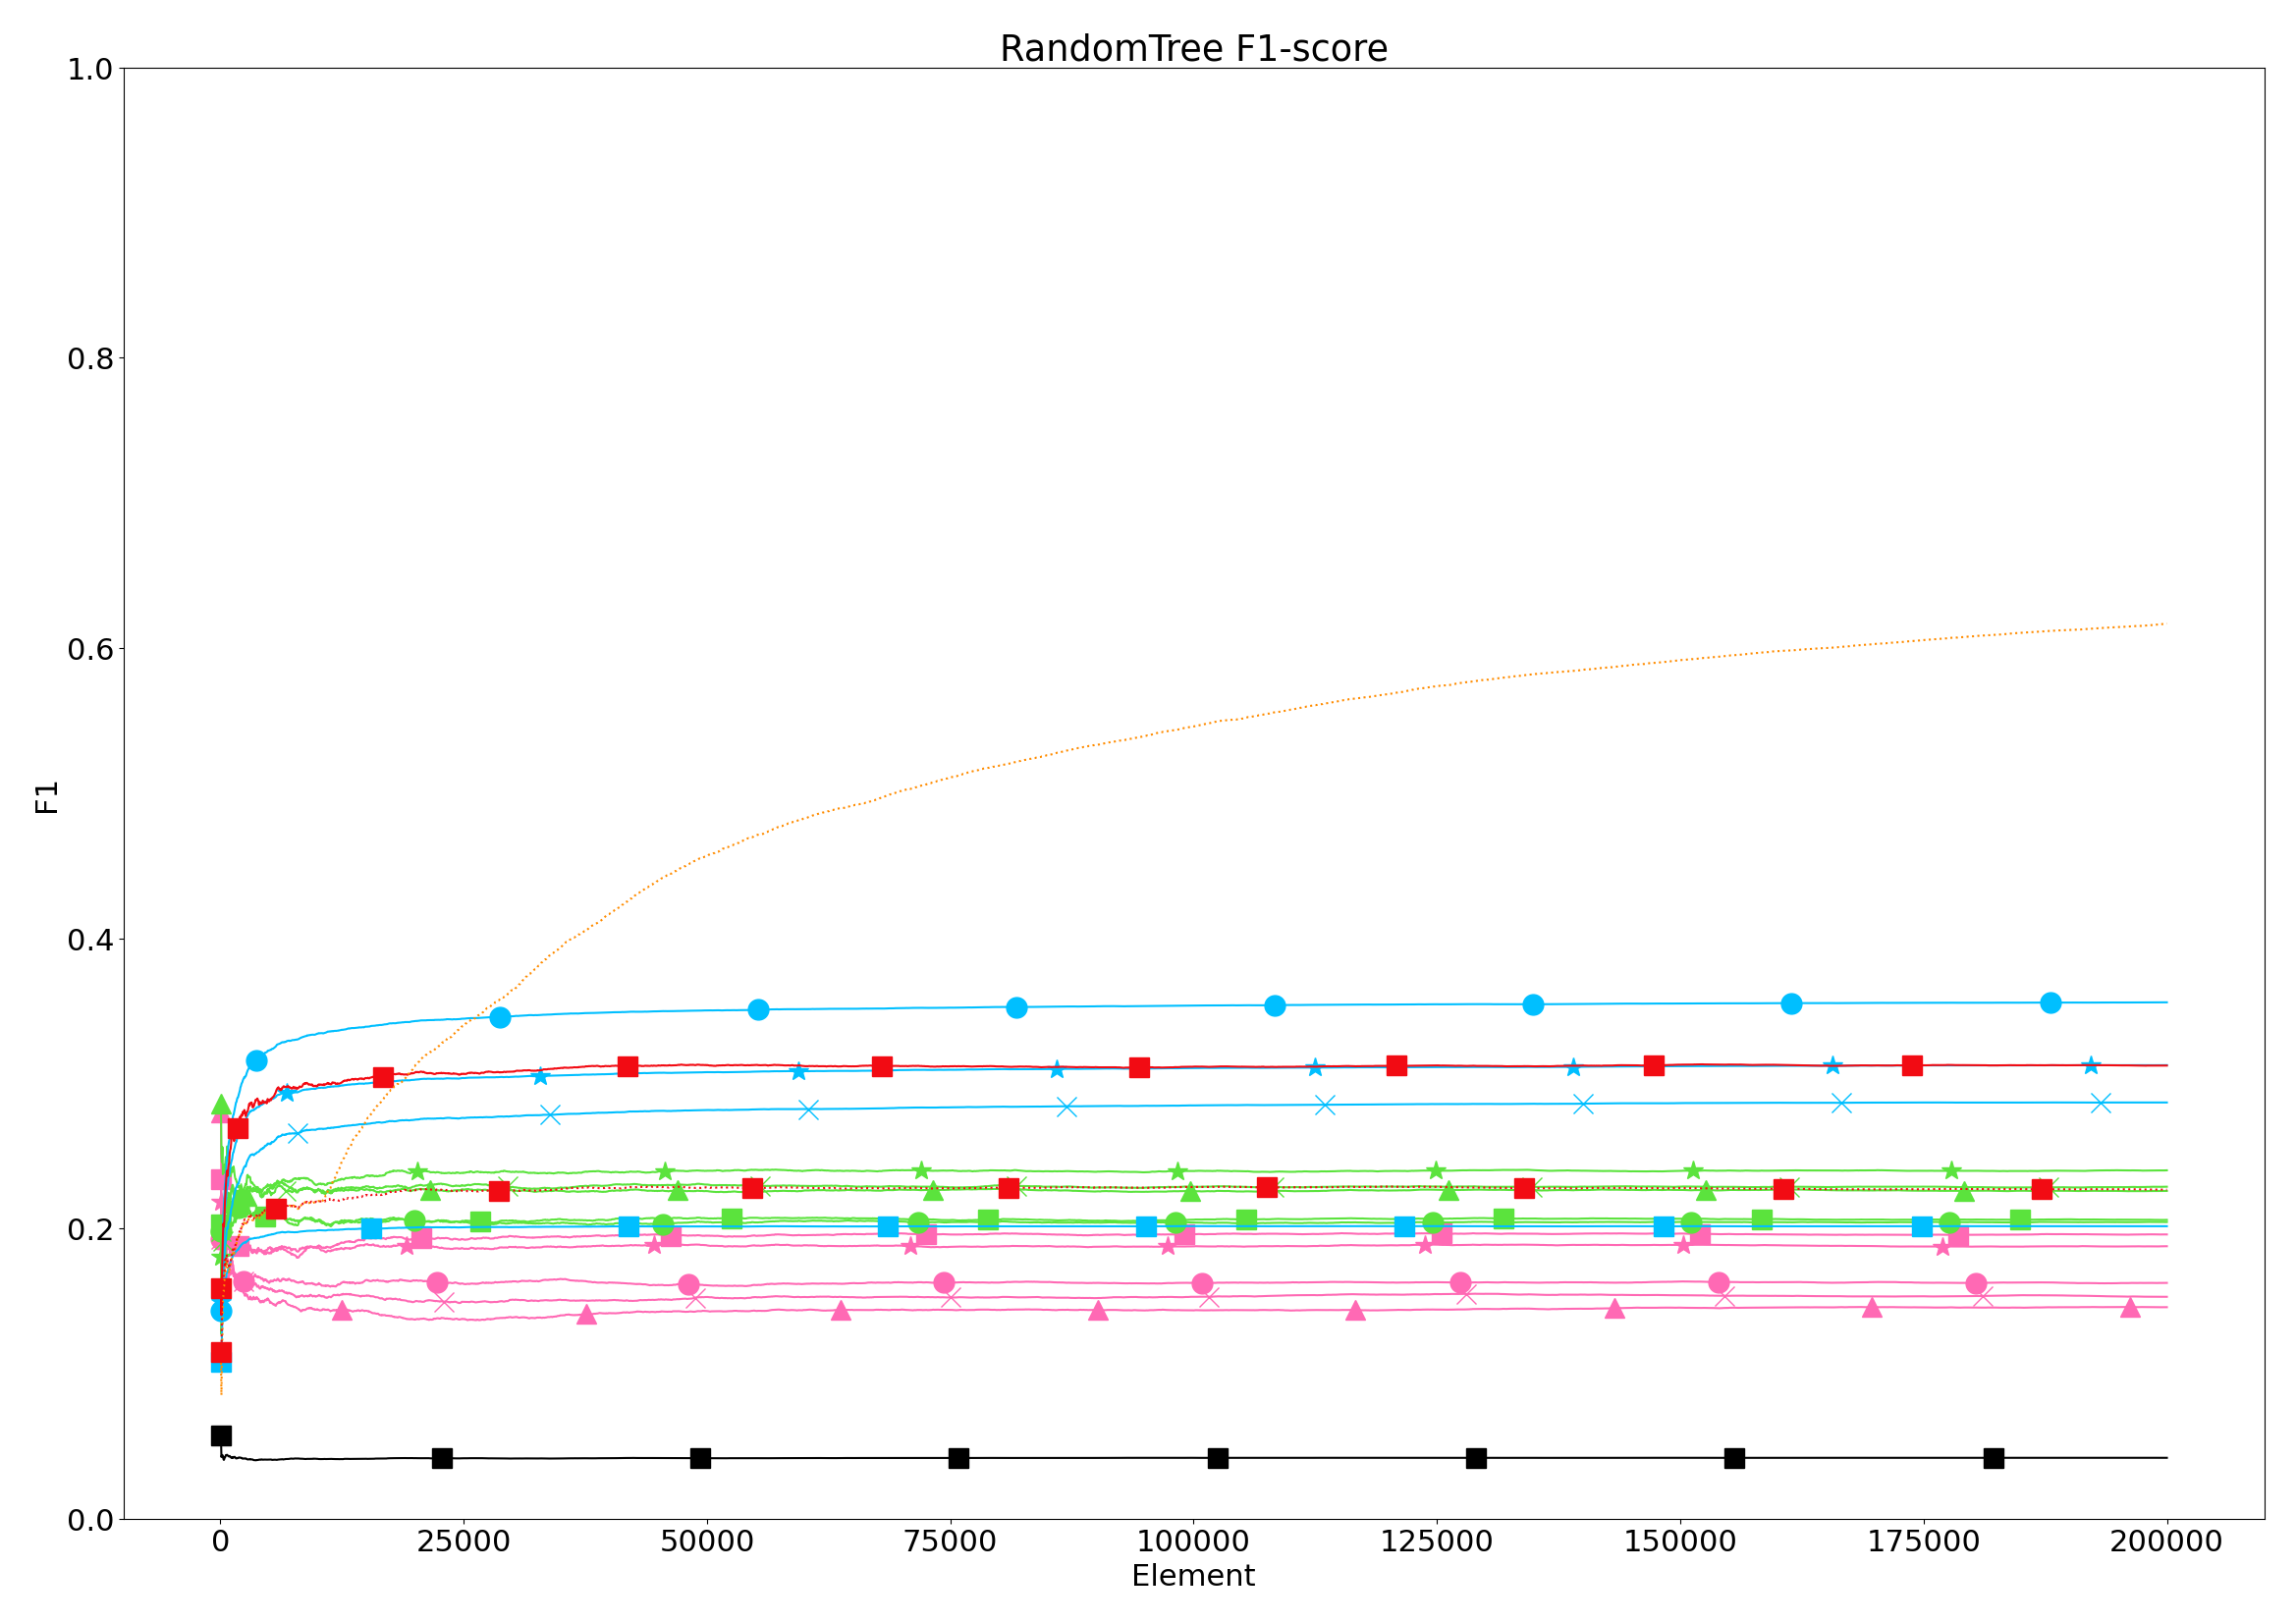
\includegraphics[width=\linewidth]{figures/results/dataset_3_f1.png}
		\caption{RandomTree}
		\label{fig:f1-dataset_3}
	\end{subfigure}
	\begin{subfigure}[t]{.5\linewidth}
		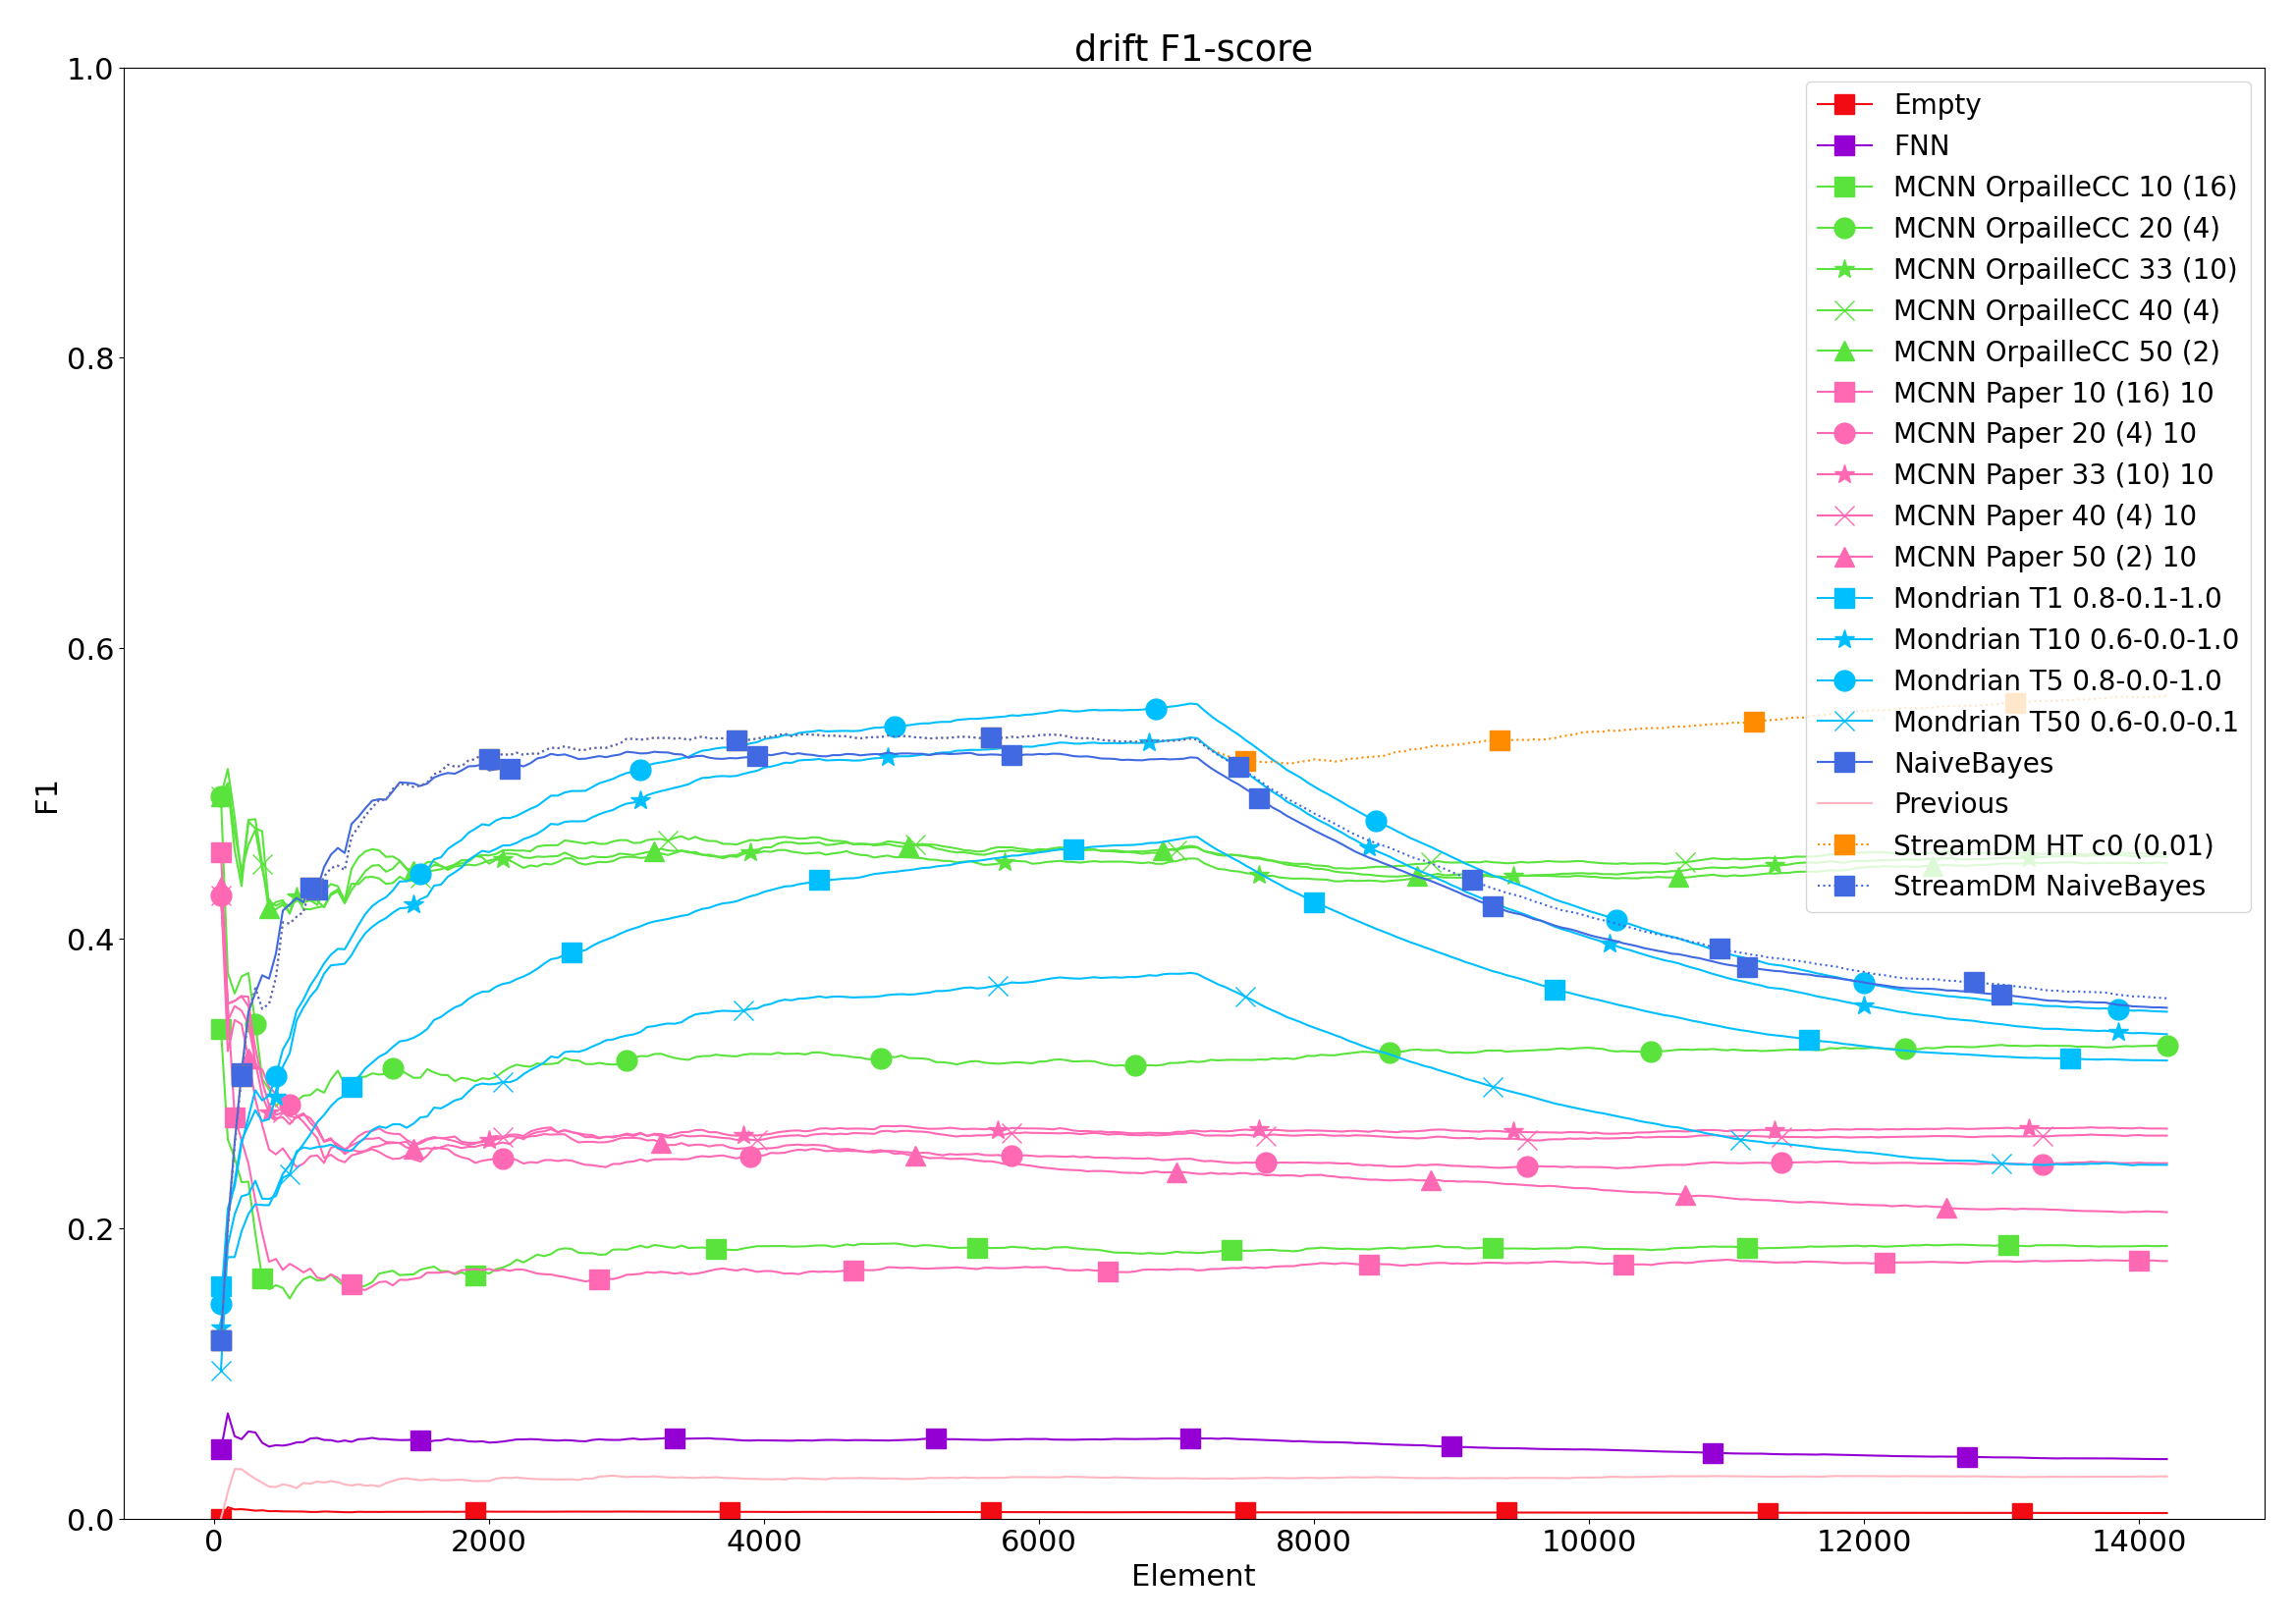
\includegraphics[width=\linewidth]{figures/results/drift_f1.png}
		\caption{Drift}
		\label{fig:f1-drift}
	\end{subfigure}

	\caption{F1-scores on each dataset.}
	\label{fig:f1}
\end{figure*}

Regarding the actual F1-scores values, we noticed wide disparities between the
datasets. On the two synthetic datsets Hyperplane and RandomRBF, Mondrian
reaches an F1-score higher than 0.95. On the other hand, with the
\banosdataset, the f1-score decreases between 0.5 and 0.6.  Finally, it barely
reaches 0.3 on \recofitdataset and RandomTree.

A similar observation can be made about the NaiveBayes classifier. Higher
F1-scores with the Hyperplane, medium performance with \banosdataset and
RandomRBF, and poor results with \recofitdataset and RandomTree.

Concerning the StreamDM HoeffdingTree algorithm, we can see that it matches
very closely the StreamDM NaiveBayes. This happens because the HoeffdingTree
uses a NaiveBayes in the leaves. However after a large number of element or
after a drift, we notice that the two start diverging because the HoeffdingTree
improves by reshaping its tree structure.

On Figure~\ref{fig:f1-banos}, there is two type of MCNN: MCNN-Origin and
MCNN-OrpailleCC.  Both algorithm are implemented in the library OrpailleCC,
however MCNN-Origin strictly follow the algorithm described in~\cite{mc-nn}
where as MCNN-OrpailleCC tweak this algorithm to ensure a fixed memory
footprint. The difference appears on how micro-clusters are removed.
MCNN-Origin removes a micro-cluster when its participation falls below a
threshold given by the user while MCNN-OrpailleCC remove the micro-cluster with
the least participation when the maximum number of micro-cluster is reached and
a new micro-cluster has to be introduced.

Figures~\ref{fig:f1} shows that in all cases, MCNN-OrpailleCC achieves
better performance than its MCNN-Origin counter-part. Additionnally, most of
the time, any MCNN-OrpailleCC performs better than all MCNN-Origin.

We note that on the real datasets (\banosdataset and \recofitdataset), the
NaiveBayes algorithm learns faster than the Mondrian. The Mondrian catches up
after a few thousand elements. Even though it is difficult to notice on most of
the datasets, we can see on \banosdataset that MCNN OrpailleCC leans faster
than the NaiveBayes when there is less than a thousand element.

Surprisingly, we observe that using 50 trees with th Mondrian algorithm show worse
f1-scores than using 5 or 10. This unexpected results appears because the
Mondrian implementation forces a fixed memory footprint. Therefore, the tree
growth are blocked when there is not enought memory. Because 50 trees fill the
memory faster than 10 or 5 trees, the classifier adaptation is blocked faster,
when the trees have not learn enough from the data. However, when the memory
available is increased, using 50 trees achieve better f1-scores than using 10
trees.

Figure~\ref{fig:f1-drift} shows the F1-score when an artificial drift is
applied on the \banosdataset. We observe that the f1-score of the Mondrian
algorithm as well as the NaiveBayes suffer from the drift and they cannot adapt
to it. We also note that after a small set back, the HoeffdingTree algorithm
gets its f1-score to increase again. Finally, we barely notice any change on
the f1-score of the MCNNs. Only the highest MCNN (MCNN-OrpailleCC with 33, 40,
and 50 clusters) have a slight decrease.
Note that the difficulties of Mondrian to adapt to the drift can be "attribuer"
to two factors. First because Mondrian cannot change the part of the tree that
already exist even though it can reshape the tree. Second, because when the
memory limit is reach, it is not able to grow anymore, thus it cannot reshape
the tree structure.

Finally, we notice that the two NaiveBayes remain close on the two real
datasets: \banosdataset and \recofitdataset. This suggest that the two
implementation are similar, but SreamDM implements additional mechanismes.


\subsection{Power}
Figure~\ref{fig:power} show the power usage of each classifiers on four
datasets. We notice that the classifier has little impact on the
power usage which remains close to 102 watts.

\begin{figure*}
	\begin{subfigure}[t]{.5\linewidth}
		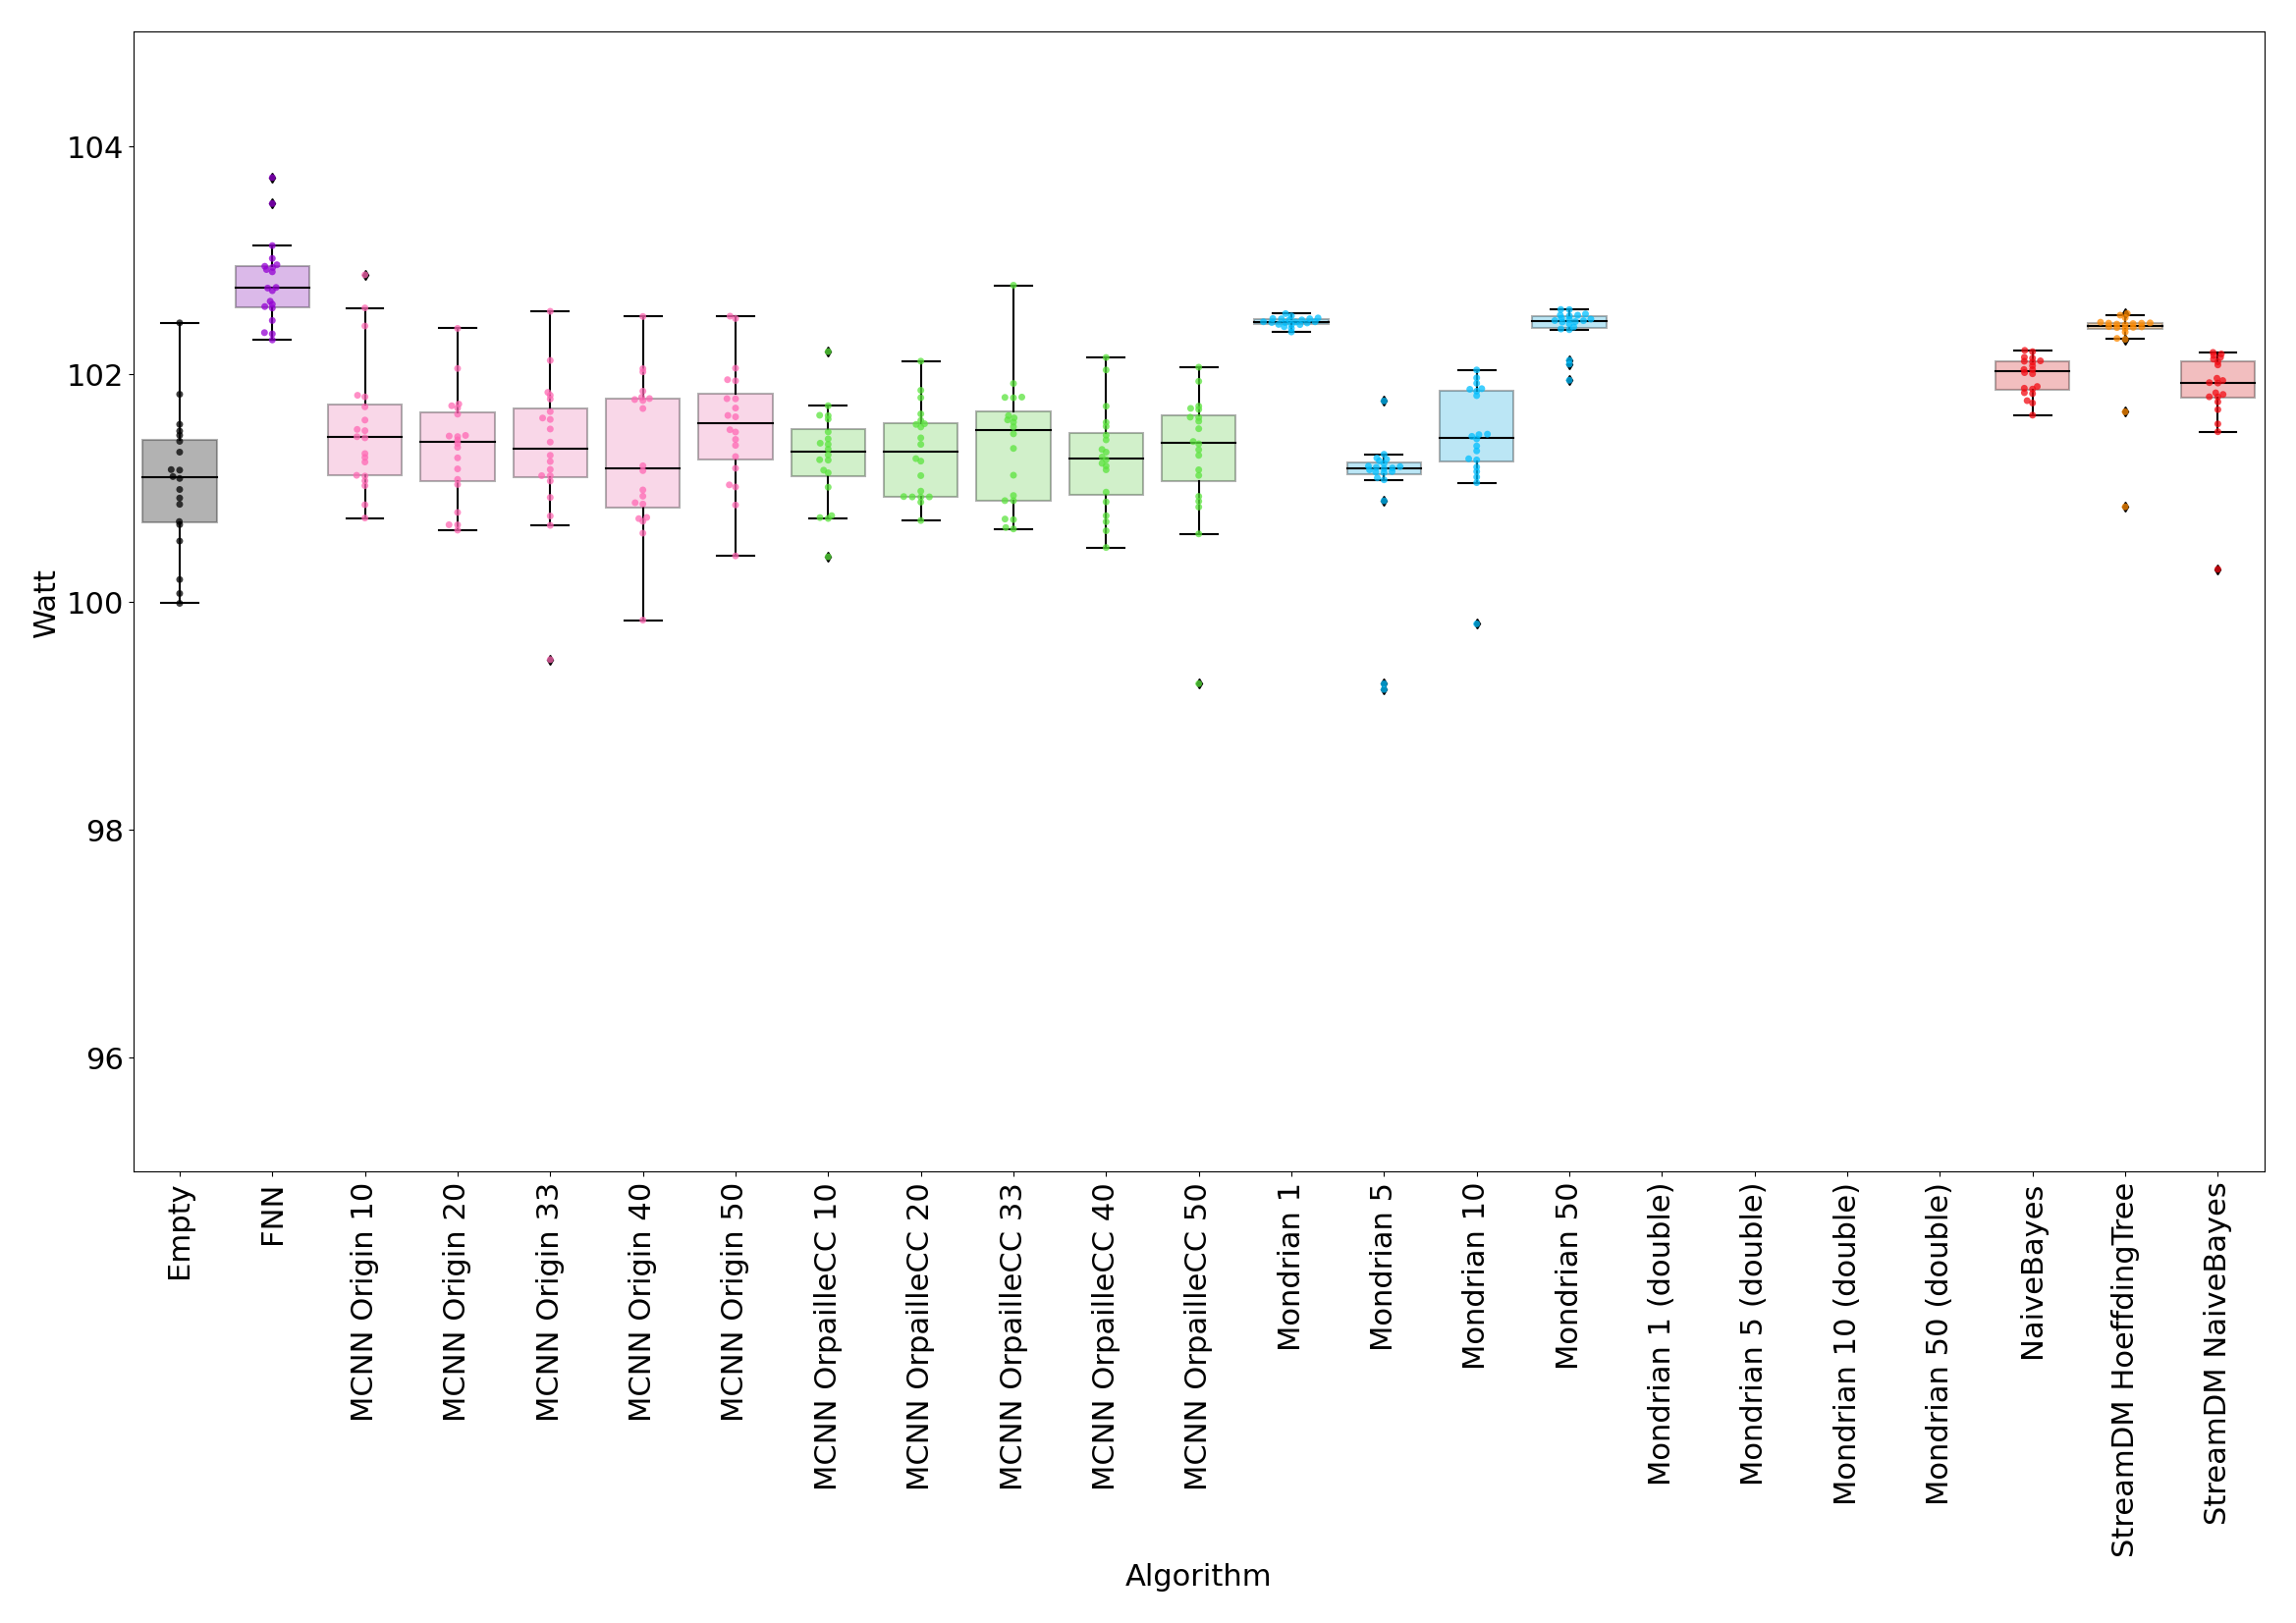
\includegraphics[width=\linewidth]{figures/results/banos_3_watt.png}
		\caption{\banosdataset}
		\label{fig:power-banos}
	\end{subfigure}
	\begin{subfigure}[t]{.5\linewidth}
		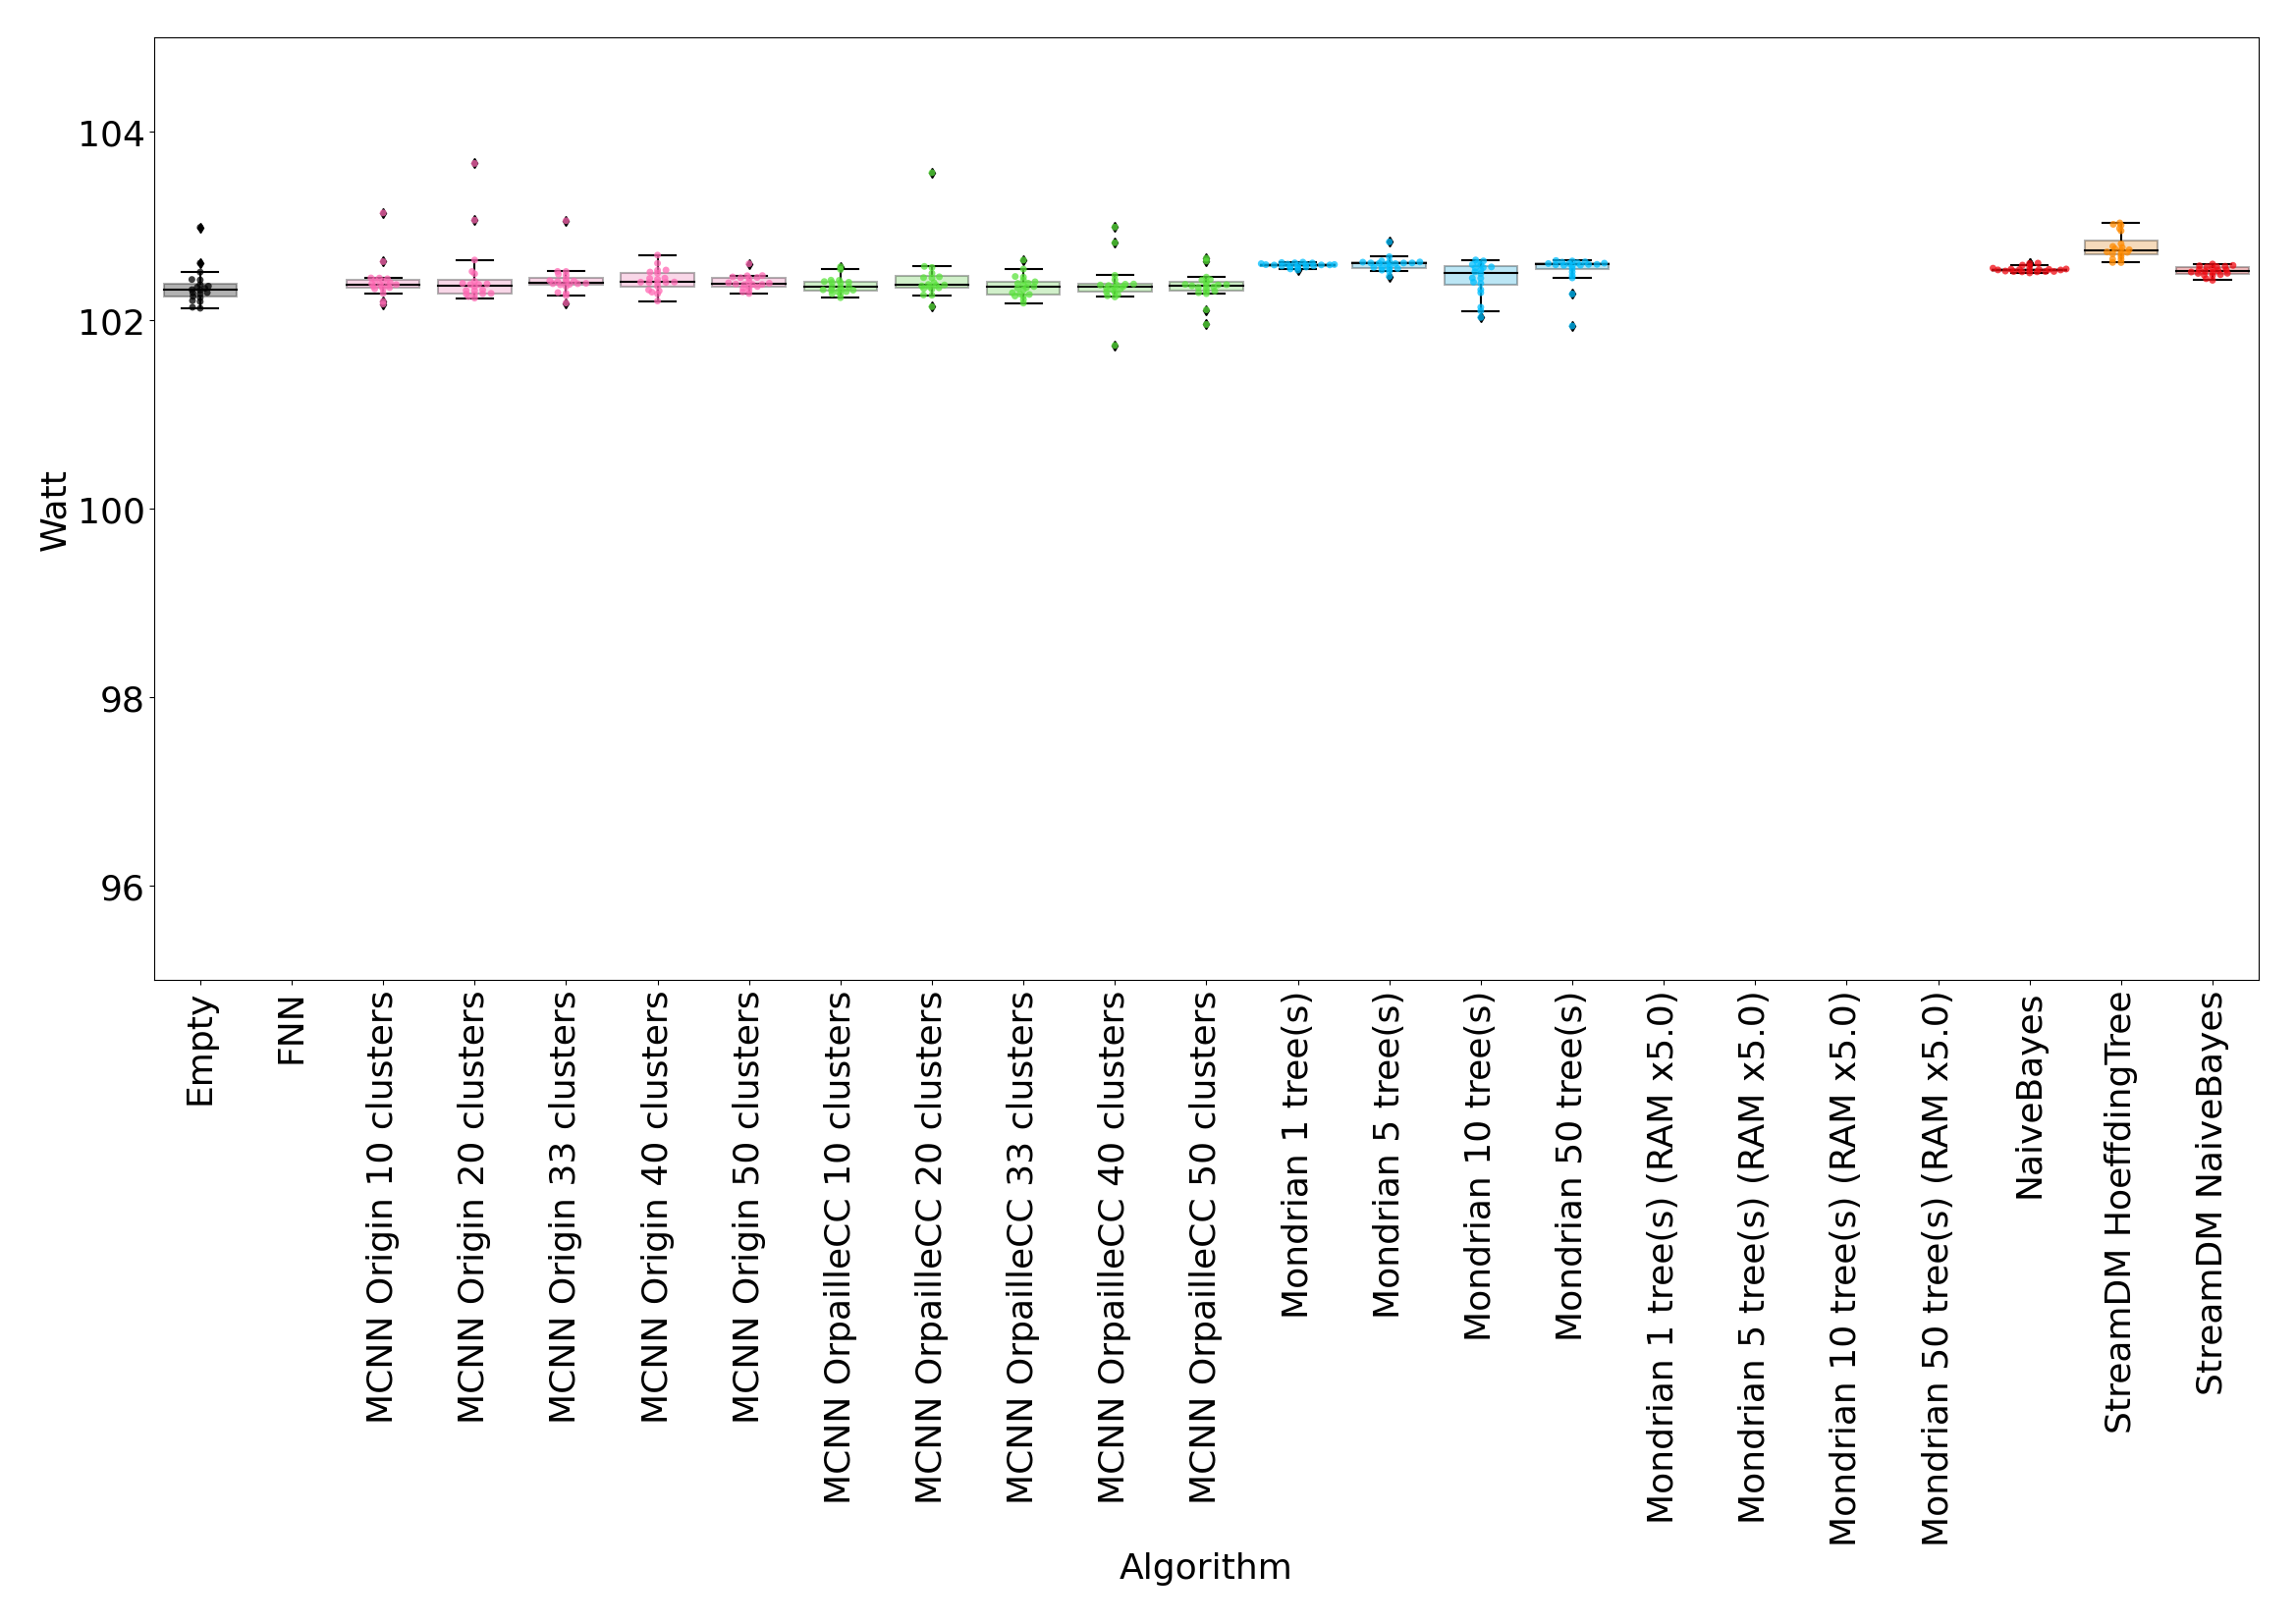
\includegraphics[width=\linewidth]{figures/results/recofit_3_watt.png}
		\caption{\recofitdataset}
		\label{fig:power-recofit}
	\end{subfigure}
	\begin{subfigure}[t]{.5\linewidth}
		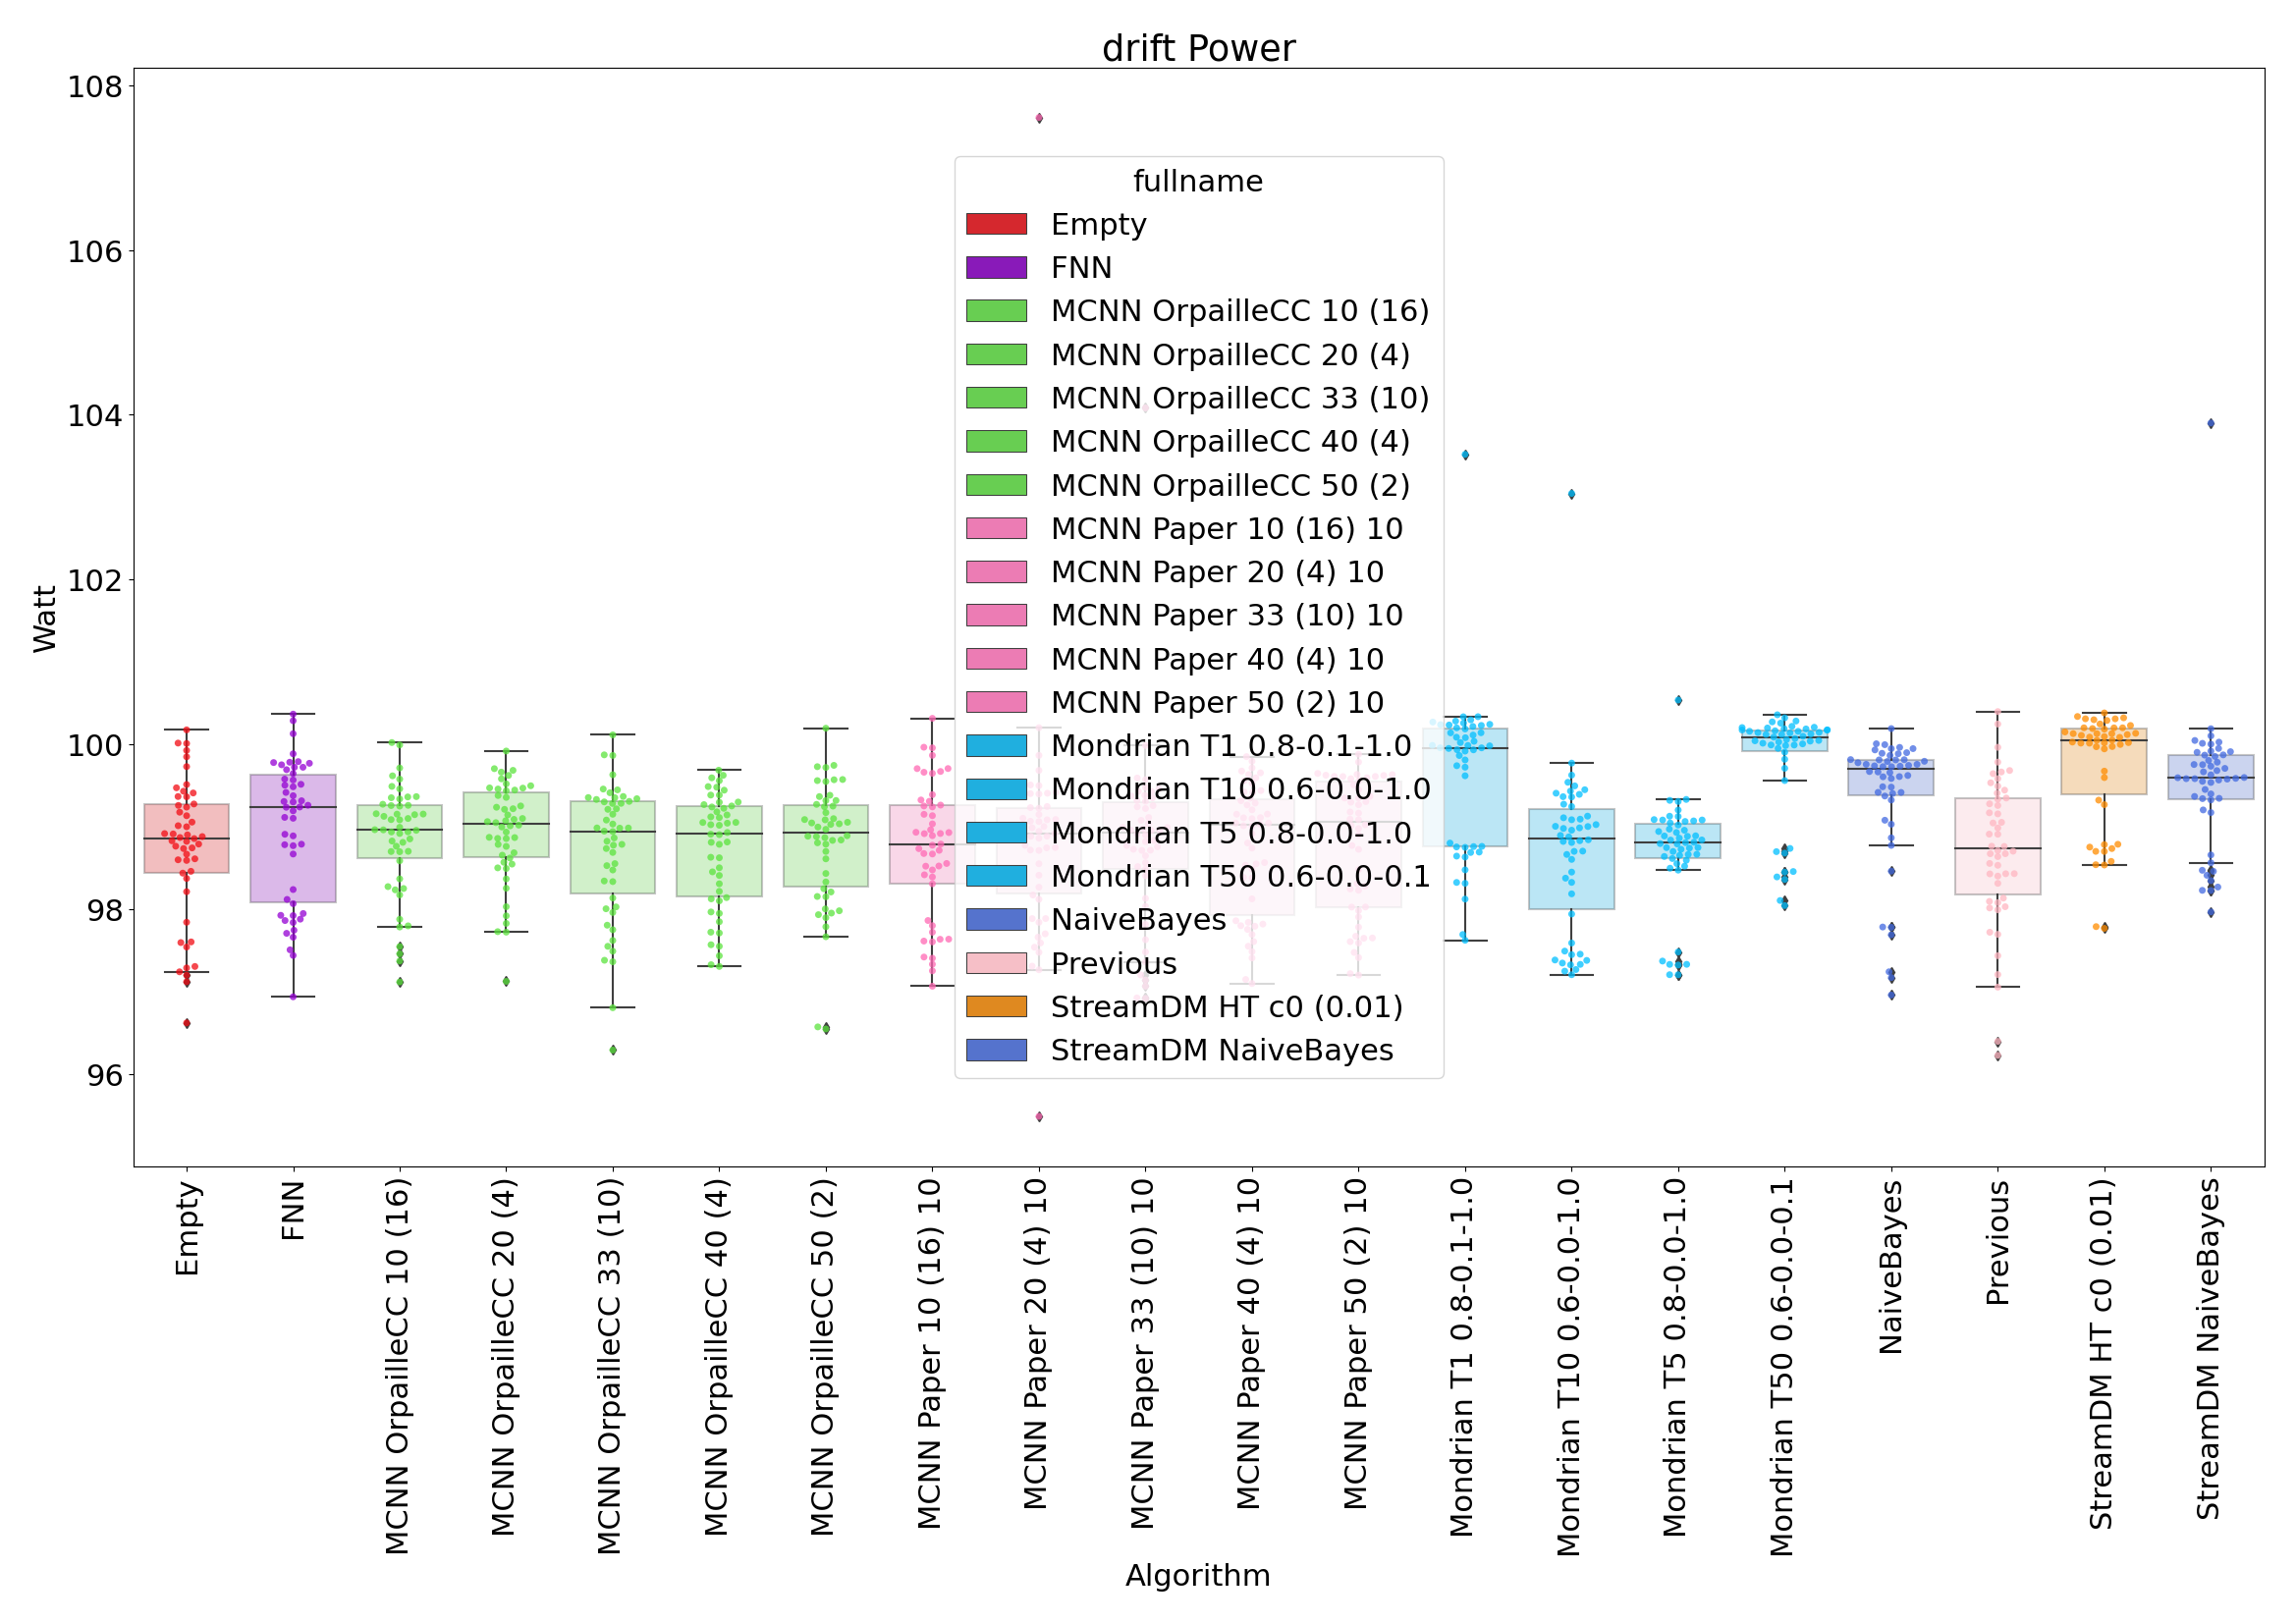
\includegraphics[width=\linewidth]{figures/results/drift_watt.png}
		\caption{\banosdataset with drift.}
		\label{fig:power-drift}
	\end{subfigure}
	\begin{subfigure}[t]{.5\linewidth}
		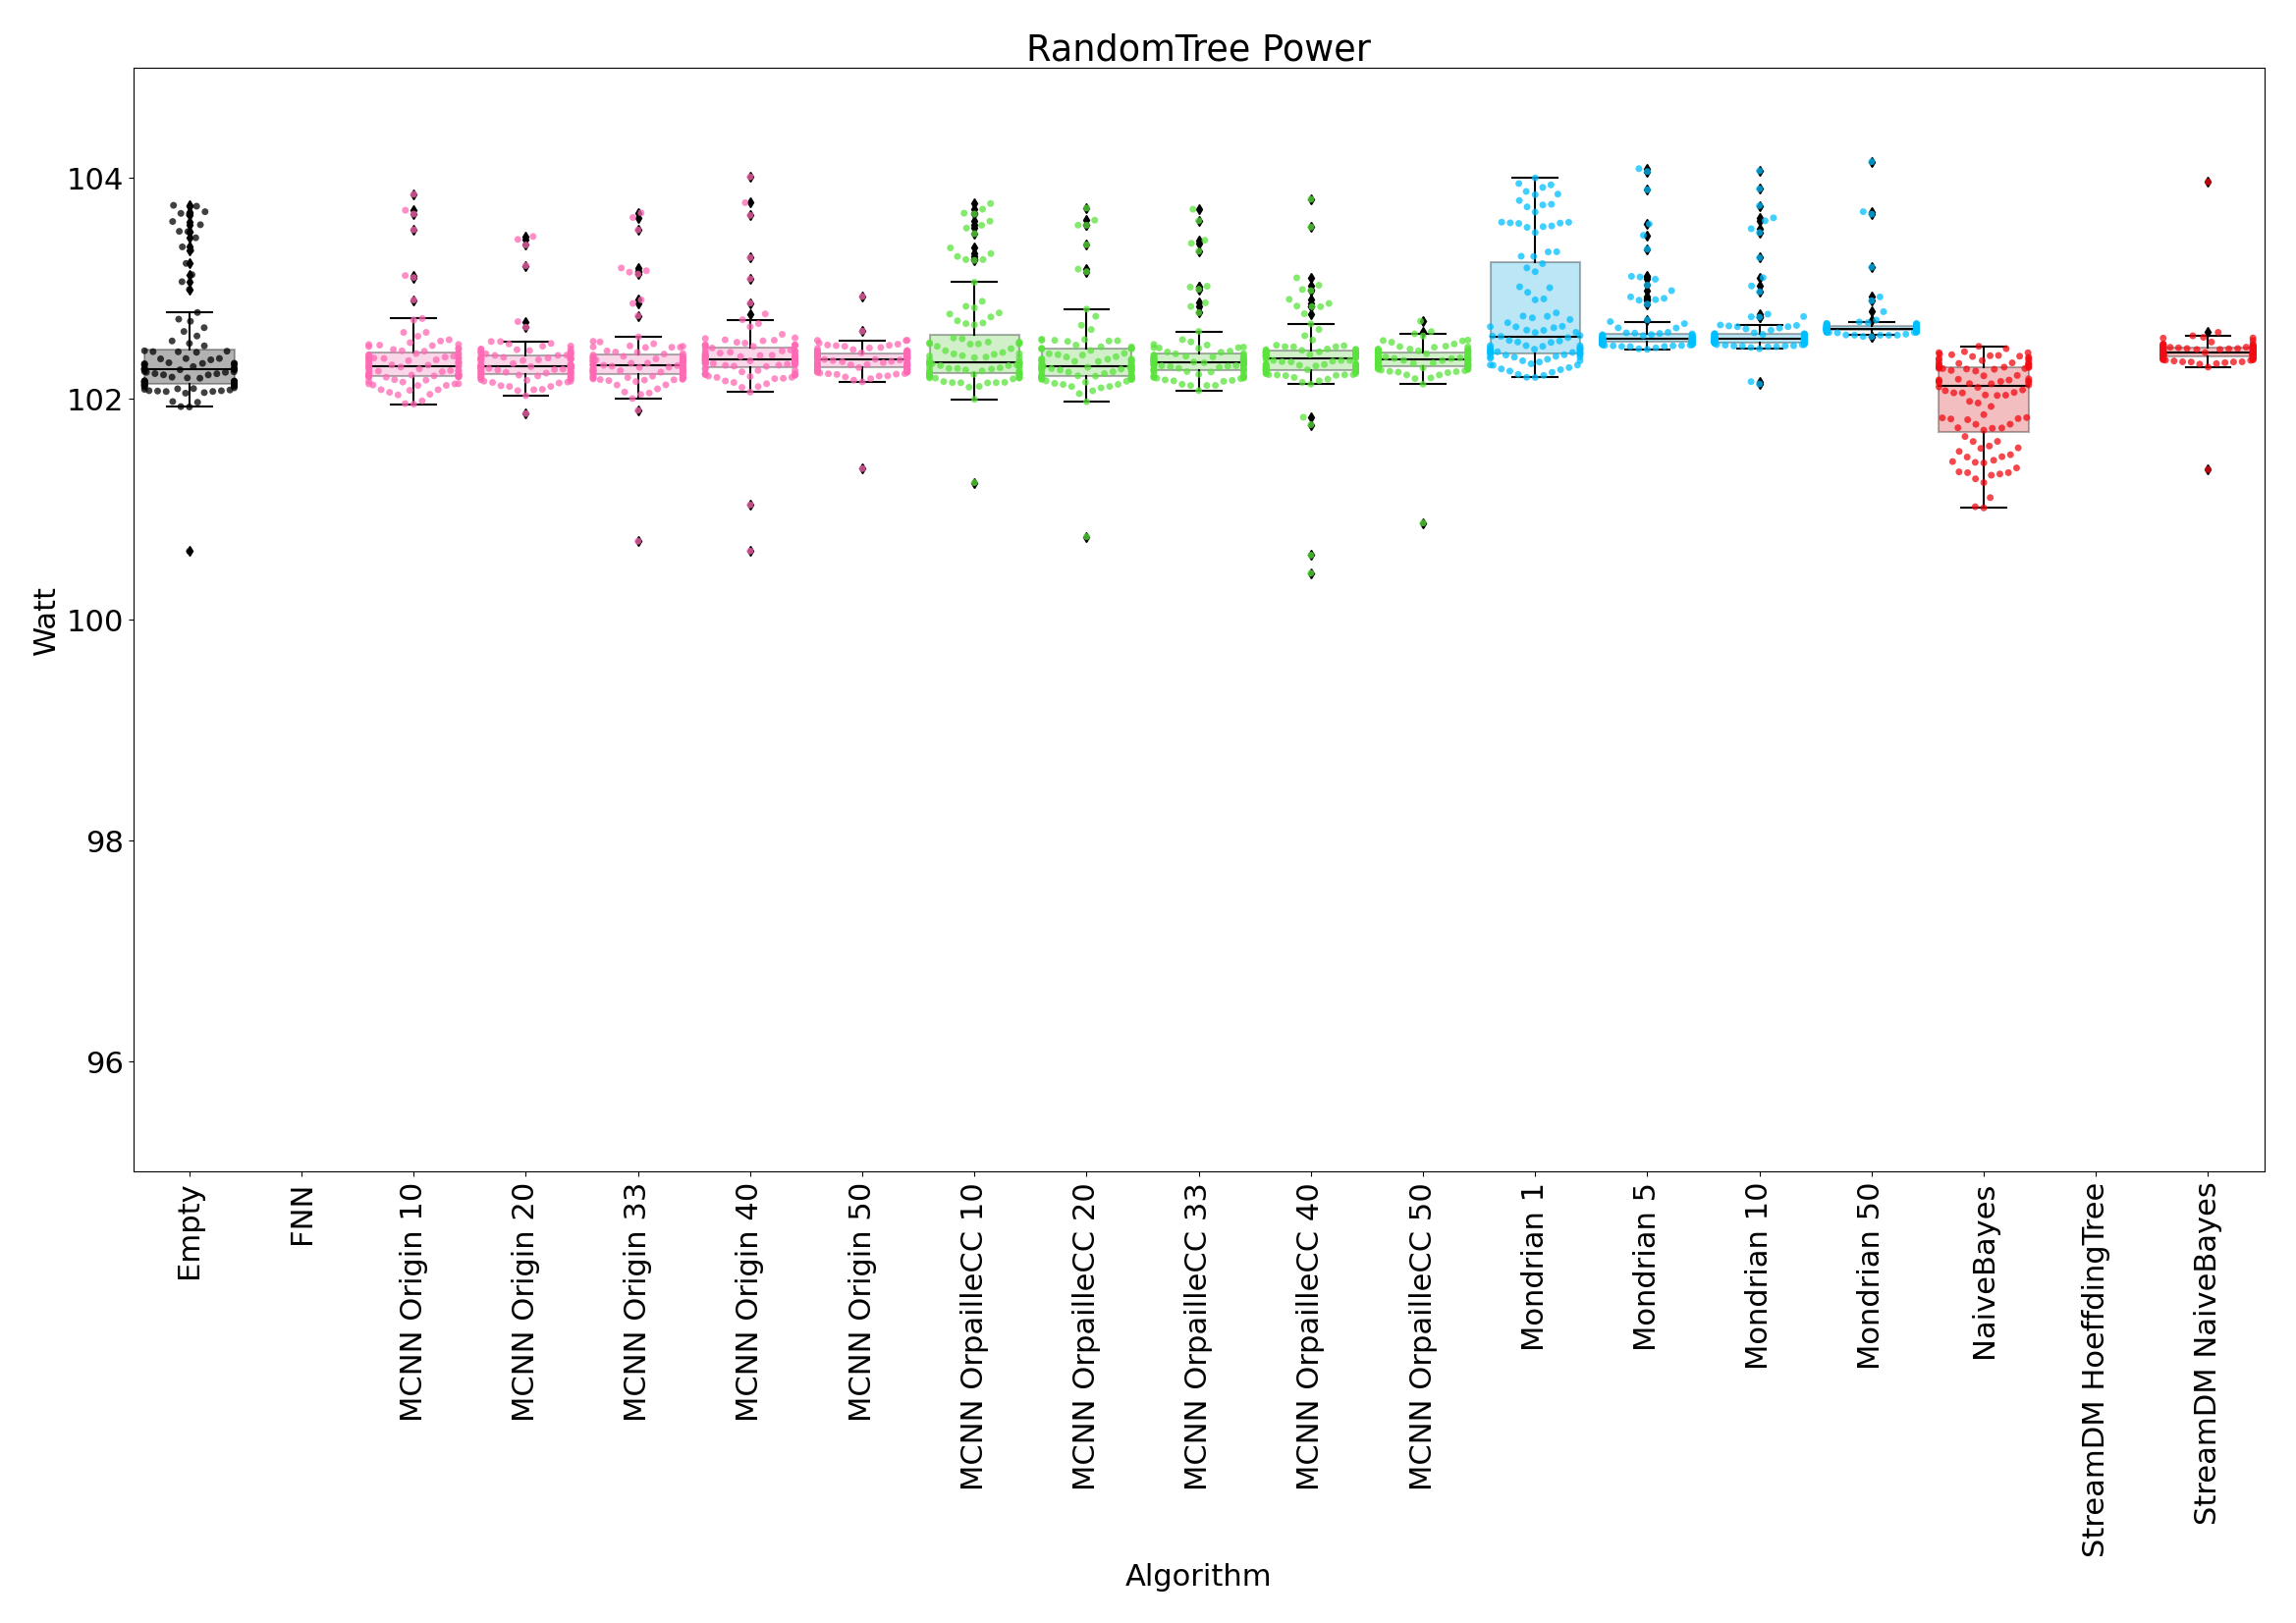
\includegraphics[width=\linewidth]{figures/results/dataset_3_watt.png}
		\caption{RandomTree}
		\label{fig:power-dataset_3}
	\end{subfigure}
	\caption{Power usage on four datasets.}
	\label{fig:power}
\end{figure*}

\subsection{Runtime}
Figure~\ref{fig:runtime} shows the runtime results on two datasets:
\banosdataset and \recofitdataset. We observe that the Mondrian algorithm is
the slowest especially with high number of trees.
It is then followed by the HoeffdingTree. Depending on the dataset, the
HoeffdingTree tree can take more time than Mondrian with 10 trees or take as
much time as Mondrian with 1 tree.

The HoeffdingTree is followed by the two NaiveBayes which are systematically
faster.  This can be explained by the NaiveBayes classifiers that run in the HoeffdingTree
leaves, so the HoeffdingTree take at least as much time as a NaiveBayes.

We observe that NaiveBayes from StreamDM is slightly faster than the one from
OrpailleCC.

Finally, the MCNNs are the fastest and they are barely noticable compare to an
empty classifier. There is still a slight difference between the MCNNs. The
more cluster we use, the slower it gets.

\begin{figure*}
	\begin{subfigure}[t]{.5\linewidth}
		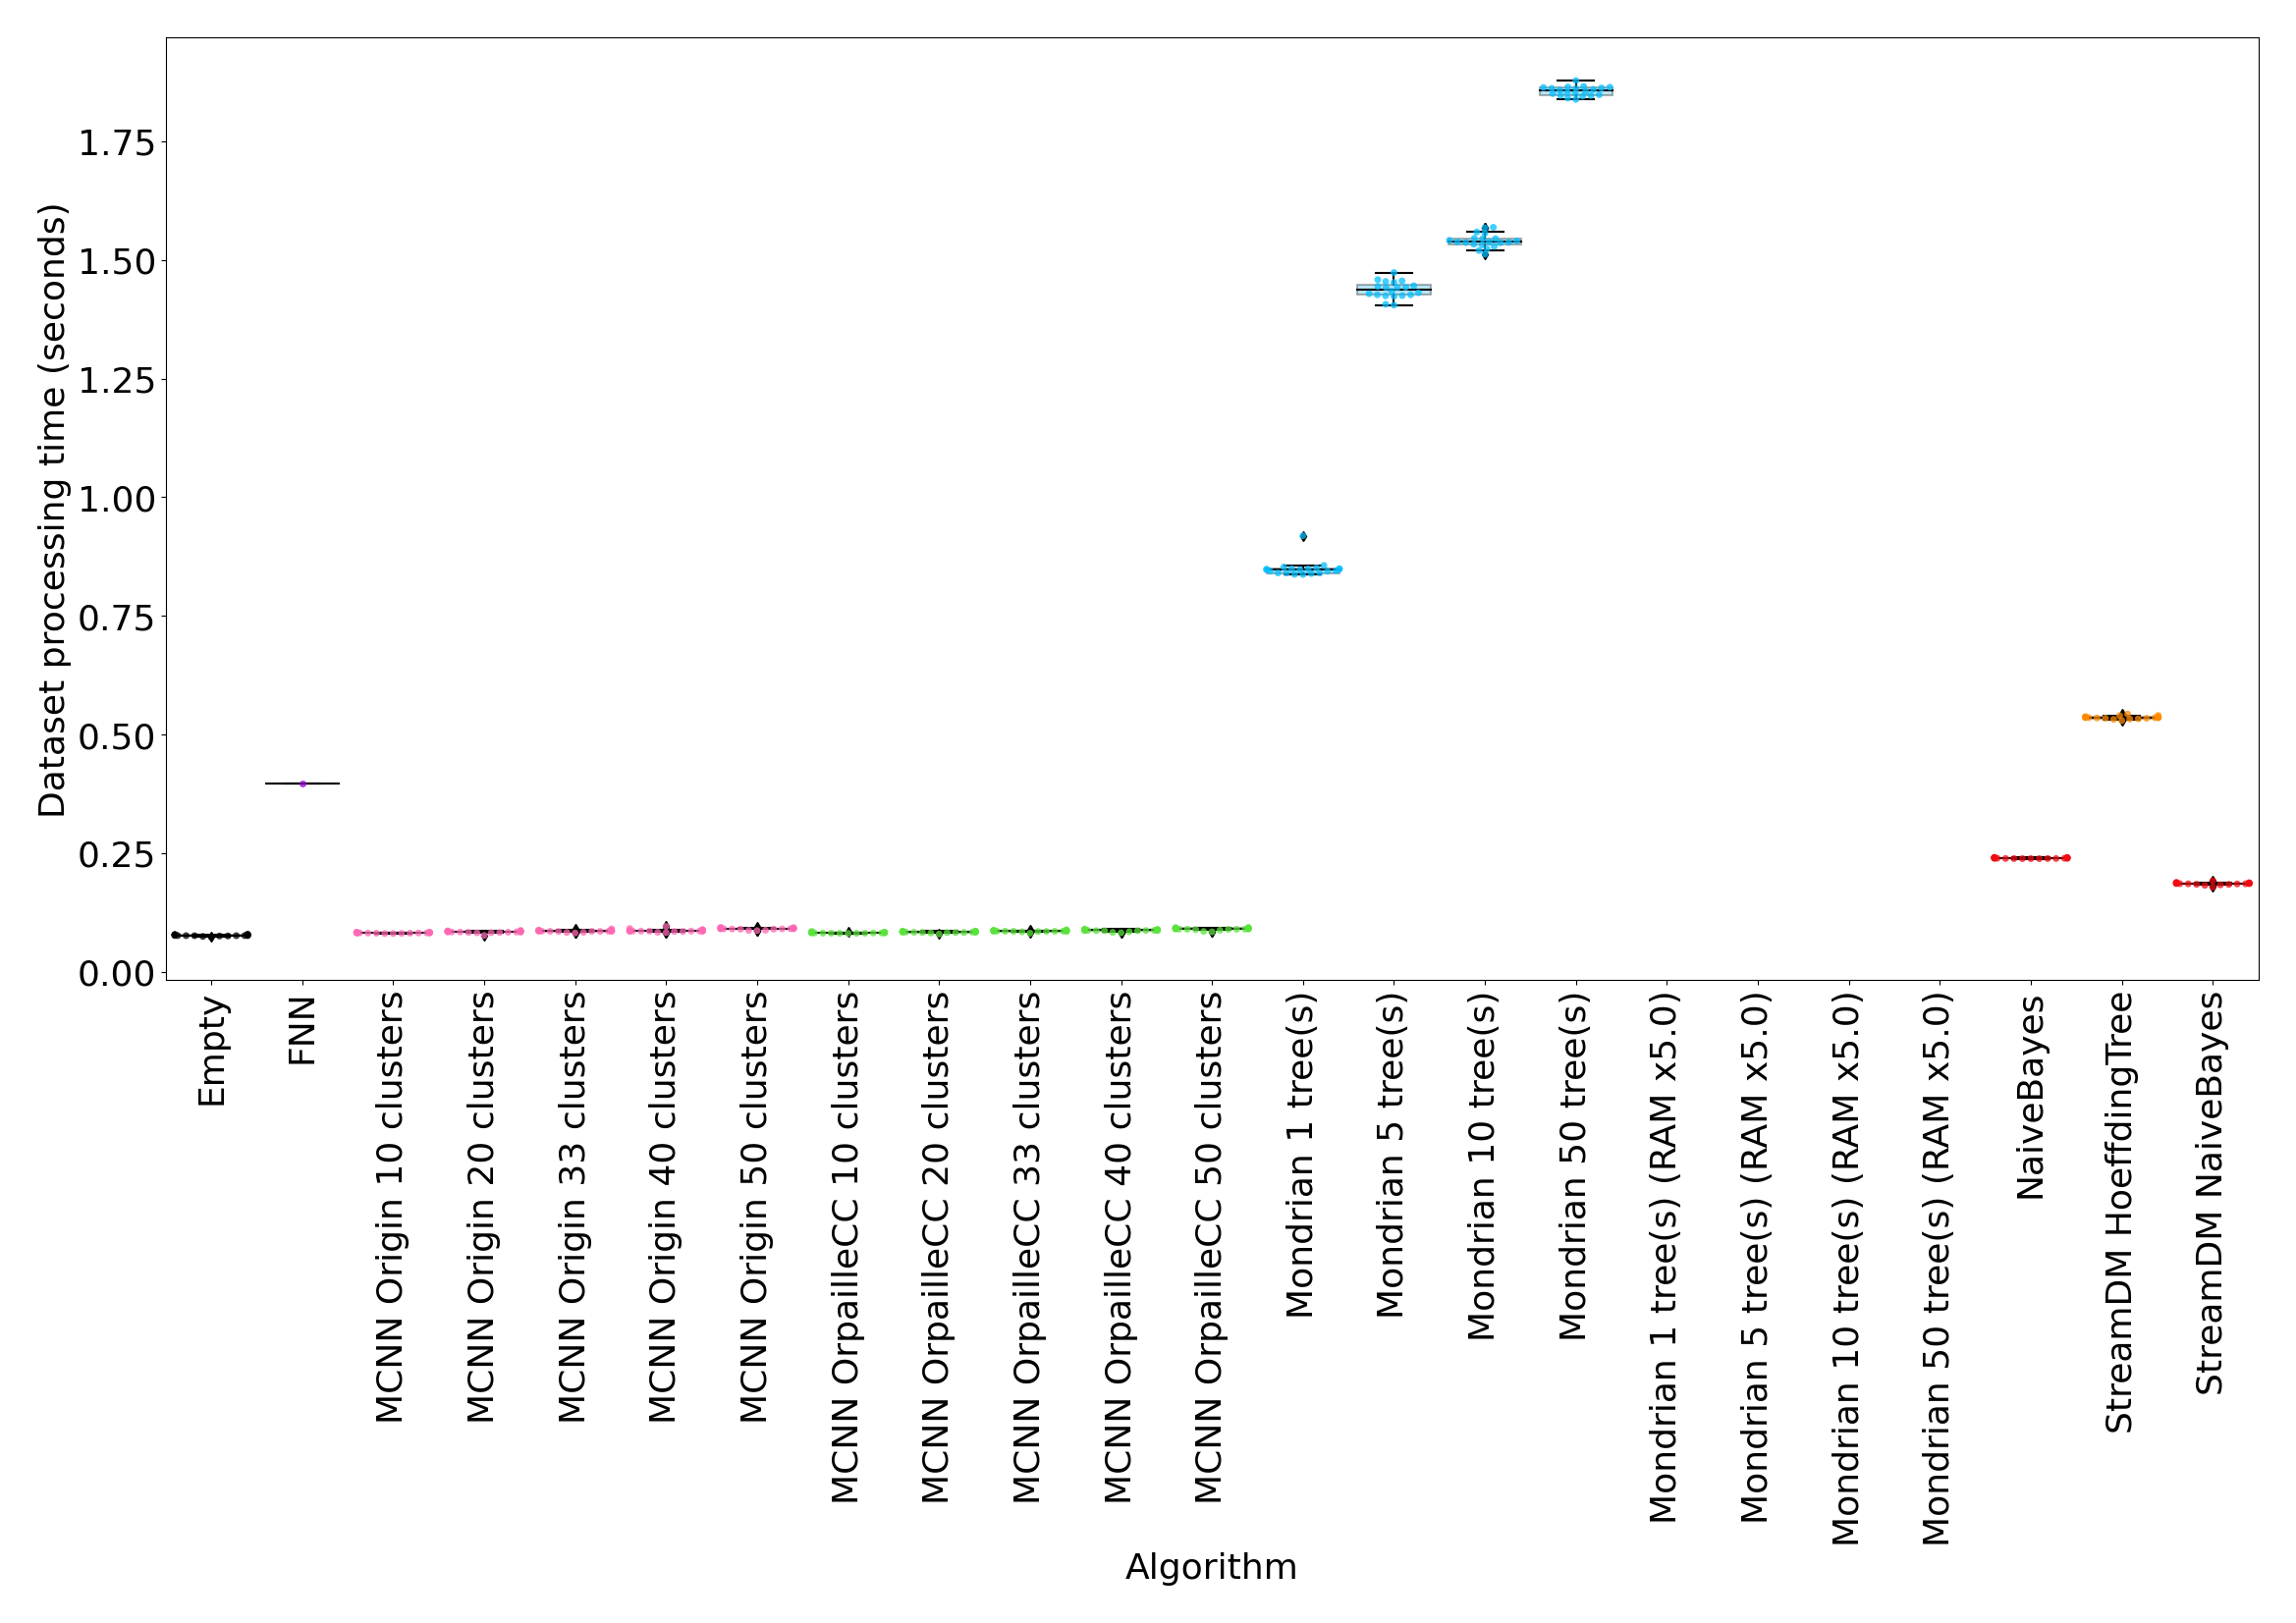
\includegraphics[width=\linewidth]{figures/results/banos_3_runtime.png}
		\caption{\banosdataset}
		\label{fig:runtime-banos}
	\end{subfigure}
	\begin{subfigure}[t]{.5\linewidth}
		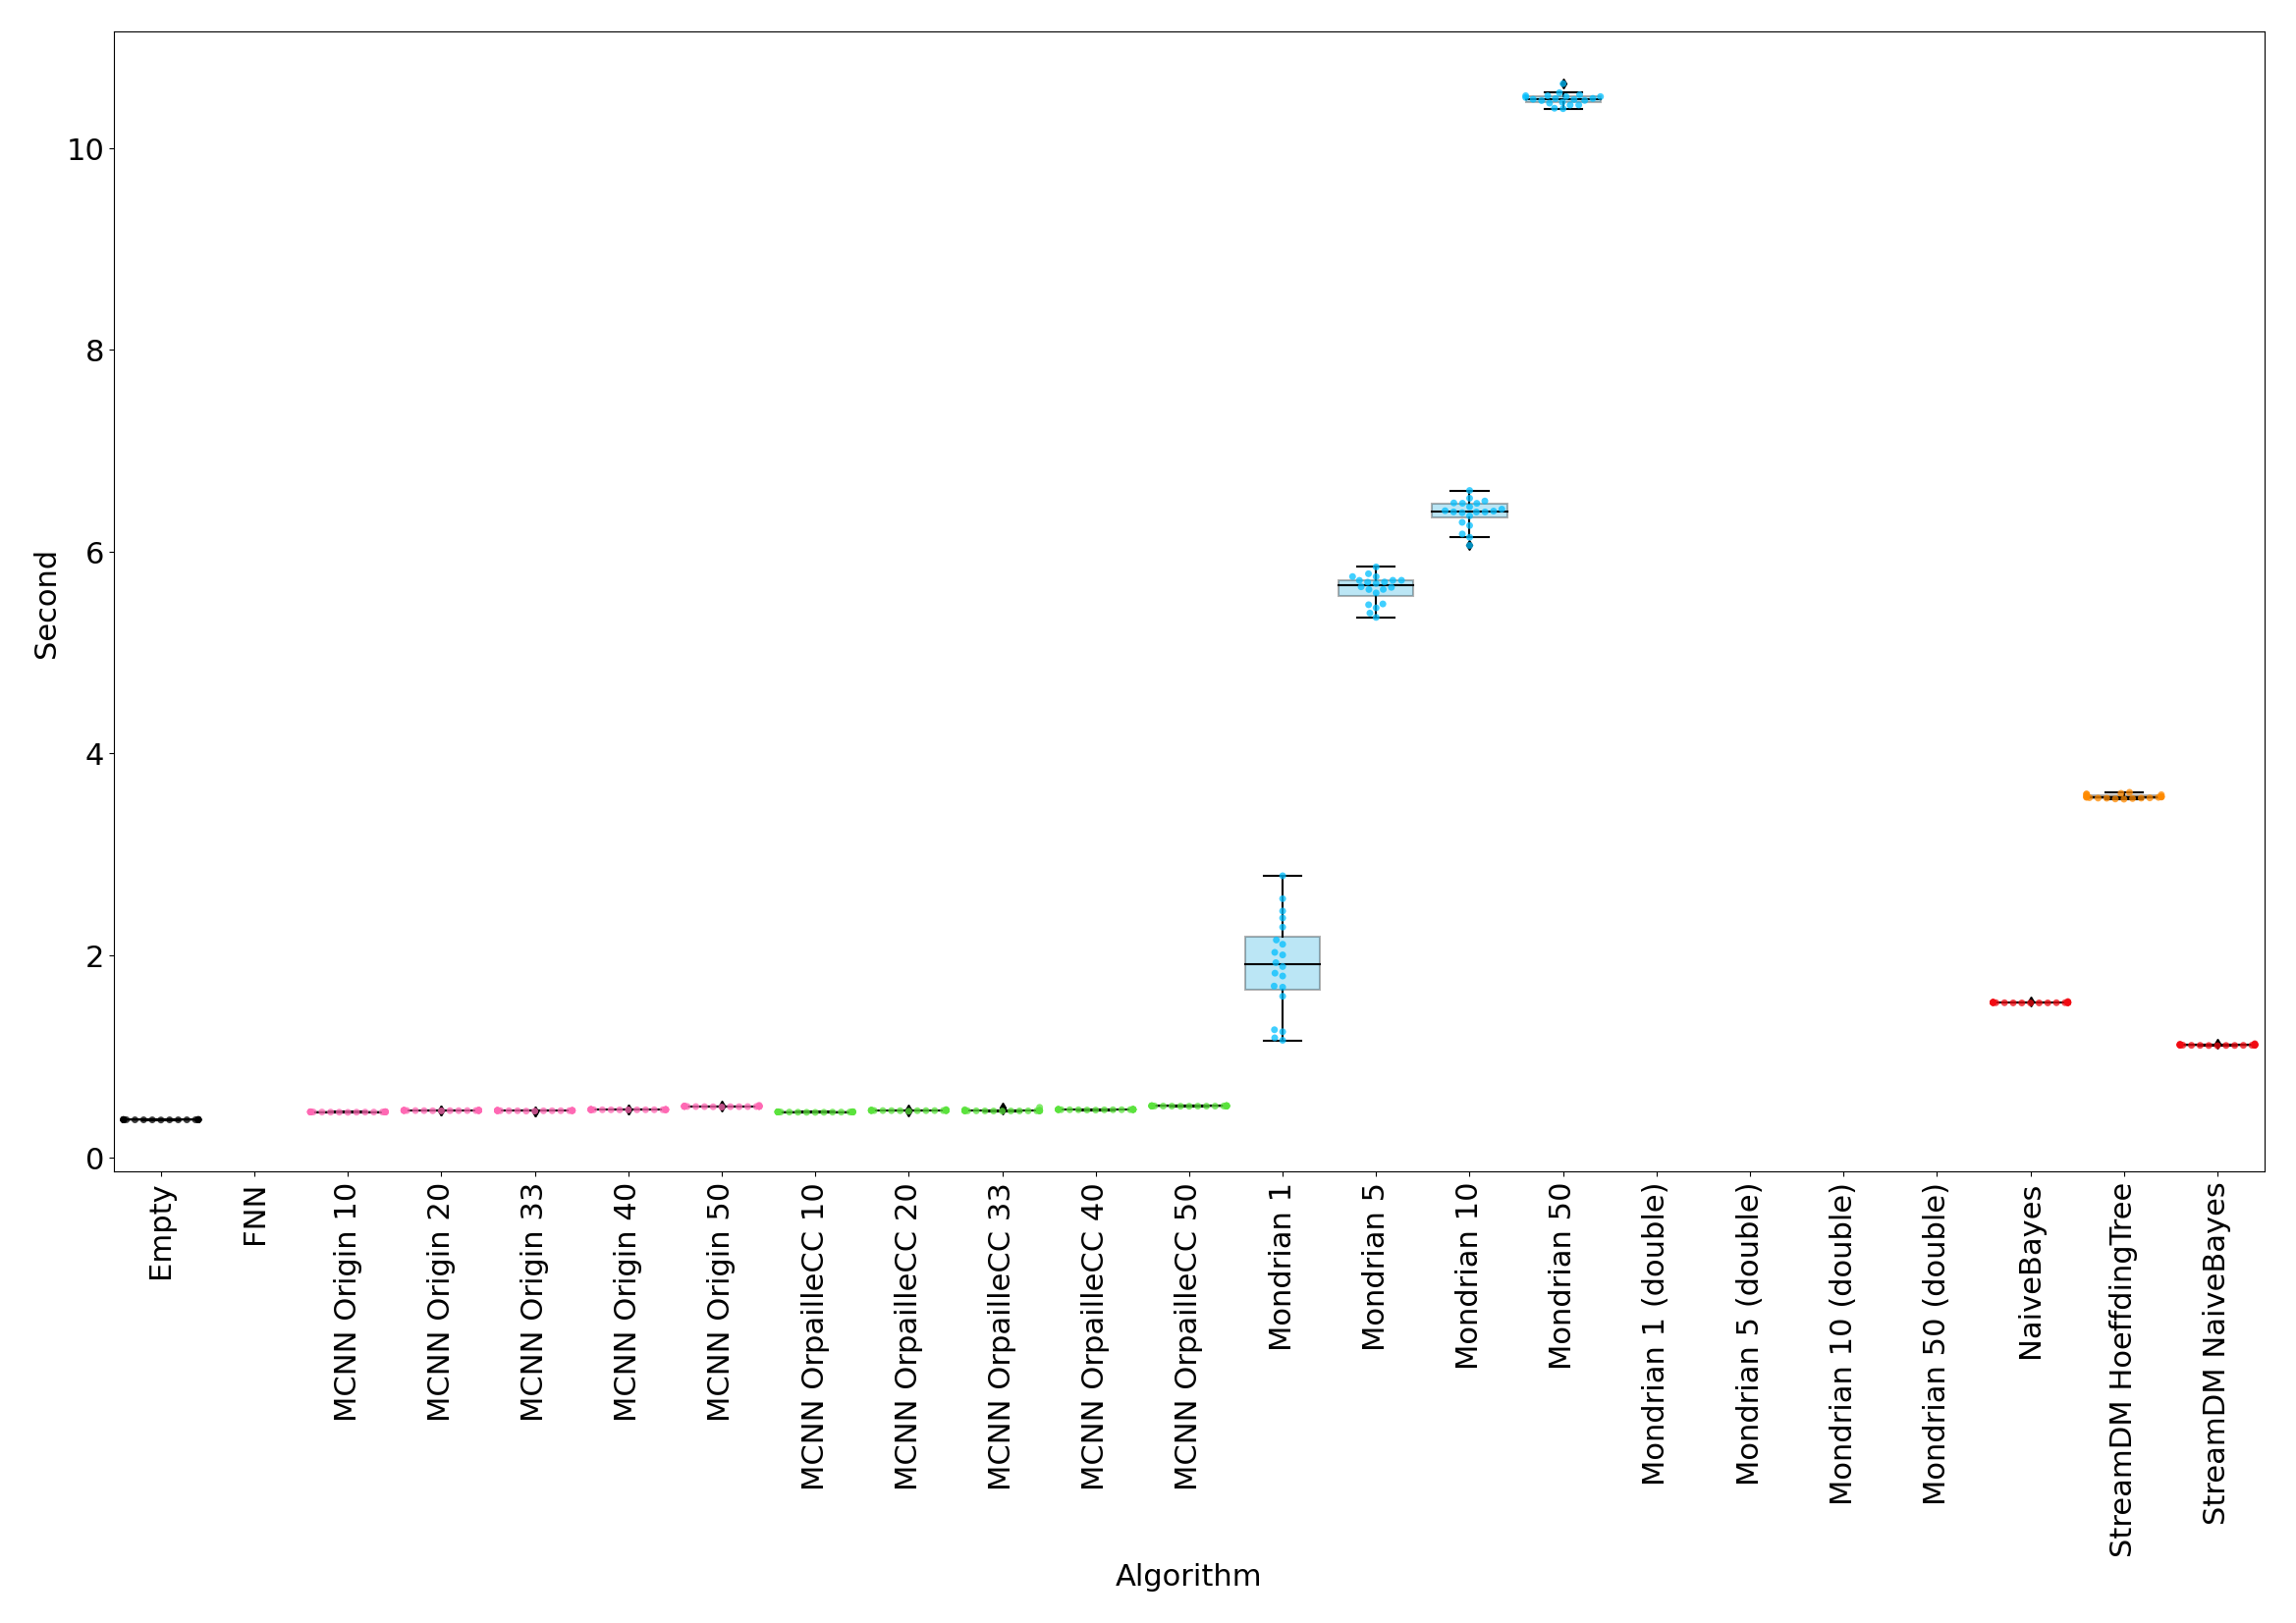
\includegraphics[width=\linewidth]{figures/results/recofit_3_runtime.png}
		\caption{\recofitdataset}
		\label{fig:runtime-recofit}
	\end{subfigure}
	\caption{Runtime with the two real datasets.}
	\label{fig:runtime}
\end{figure*}

\subsection{Memory}
Figure~\ref{fig:memory} shows the evolution of the memory footprint for the
\banosdataset.  It is similar accross all datasets because most algorithms follow
a bounded memory policy or have a constant space complexity.

\begin{figure}[H]
	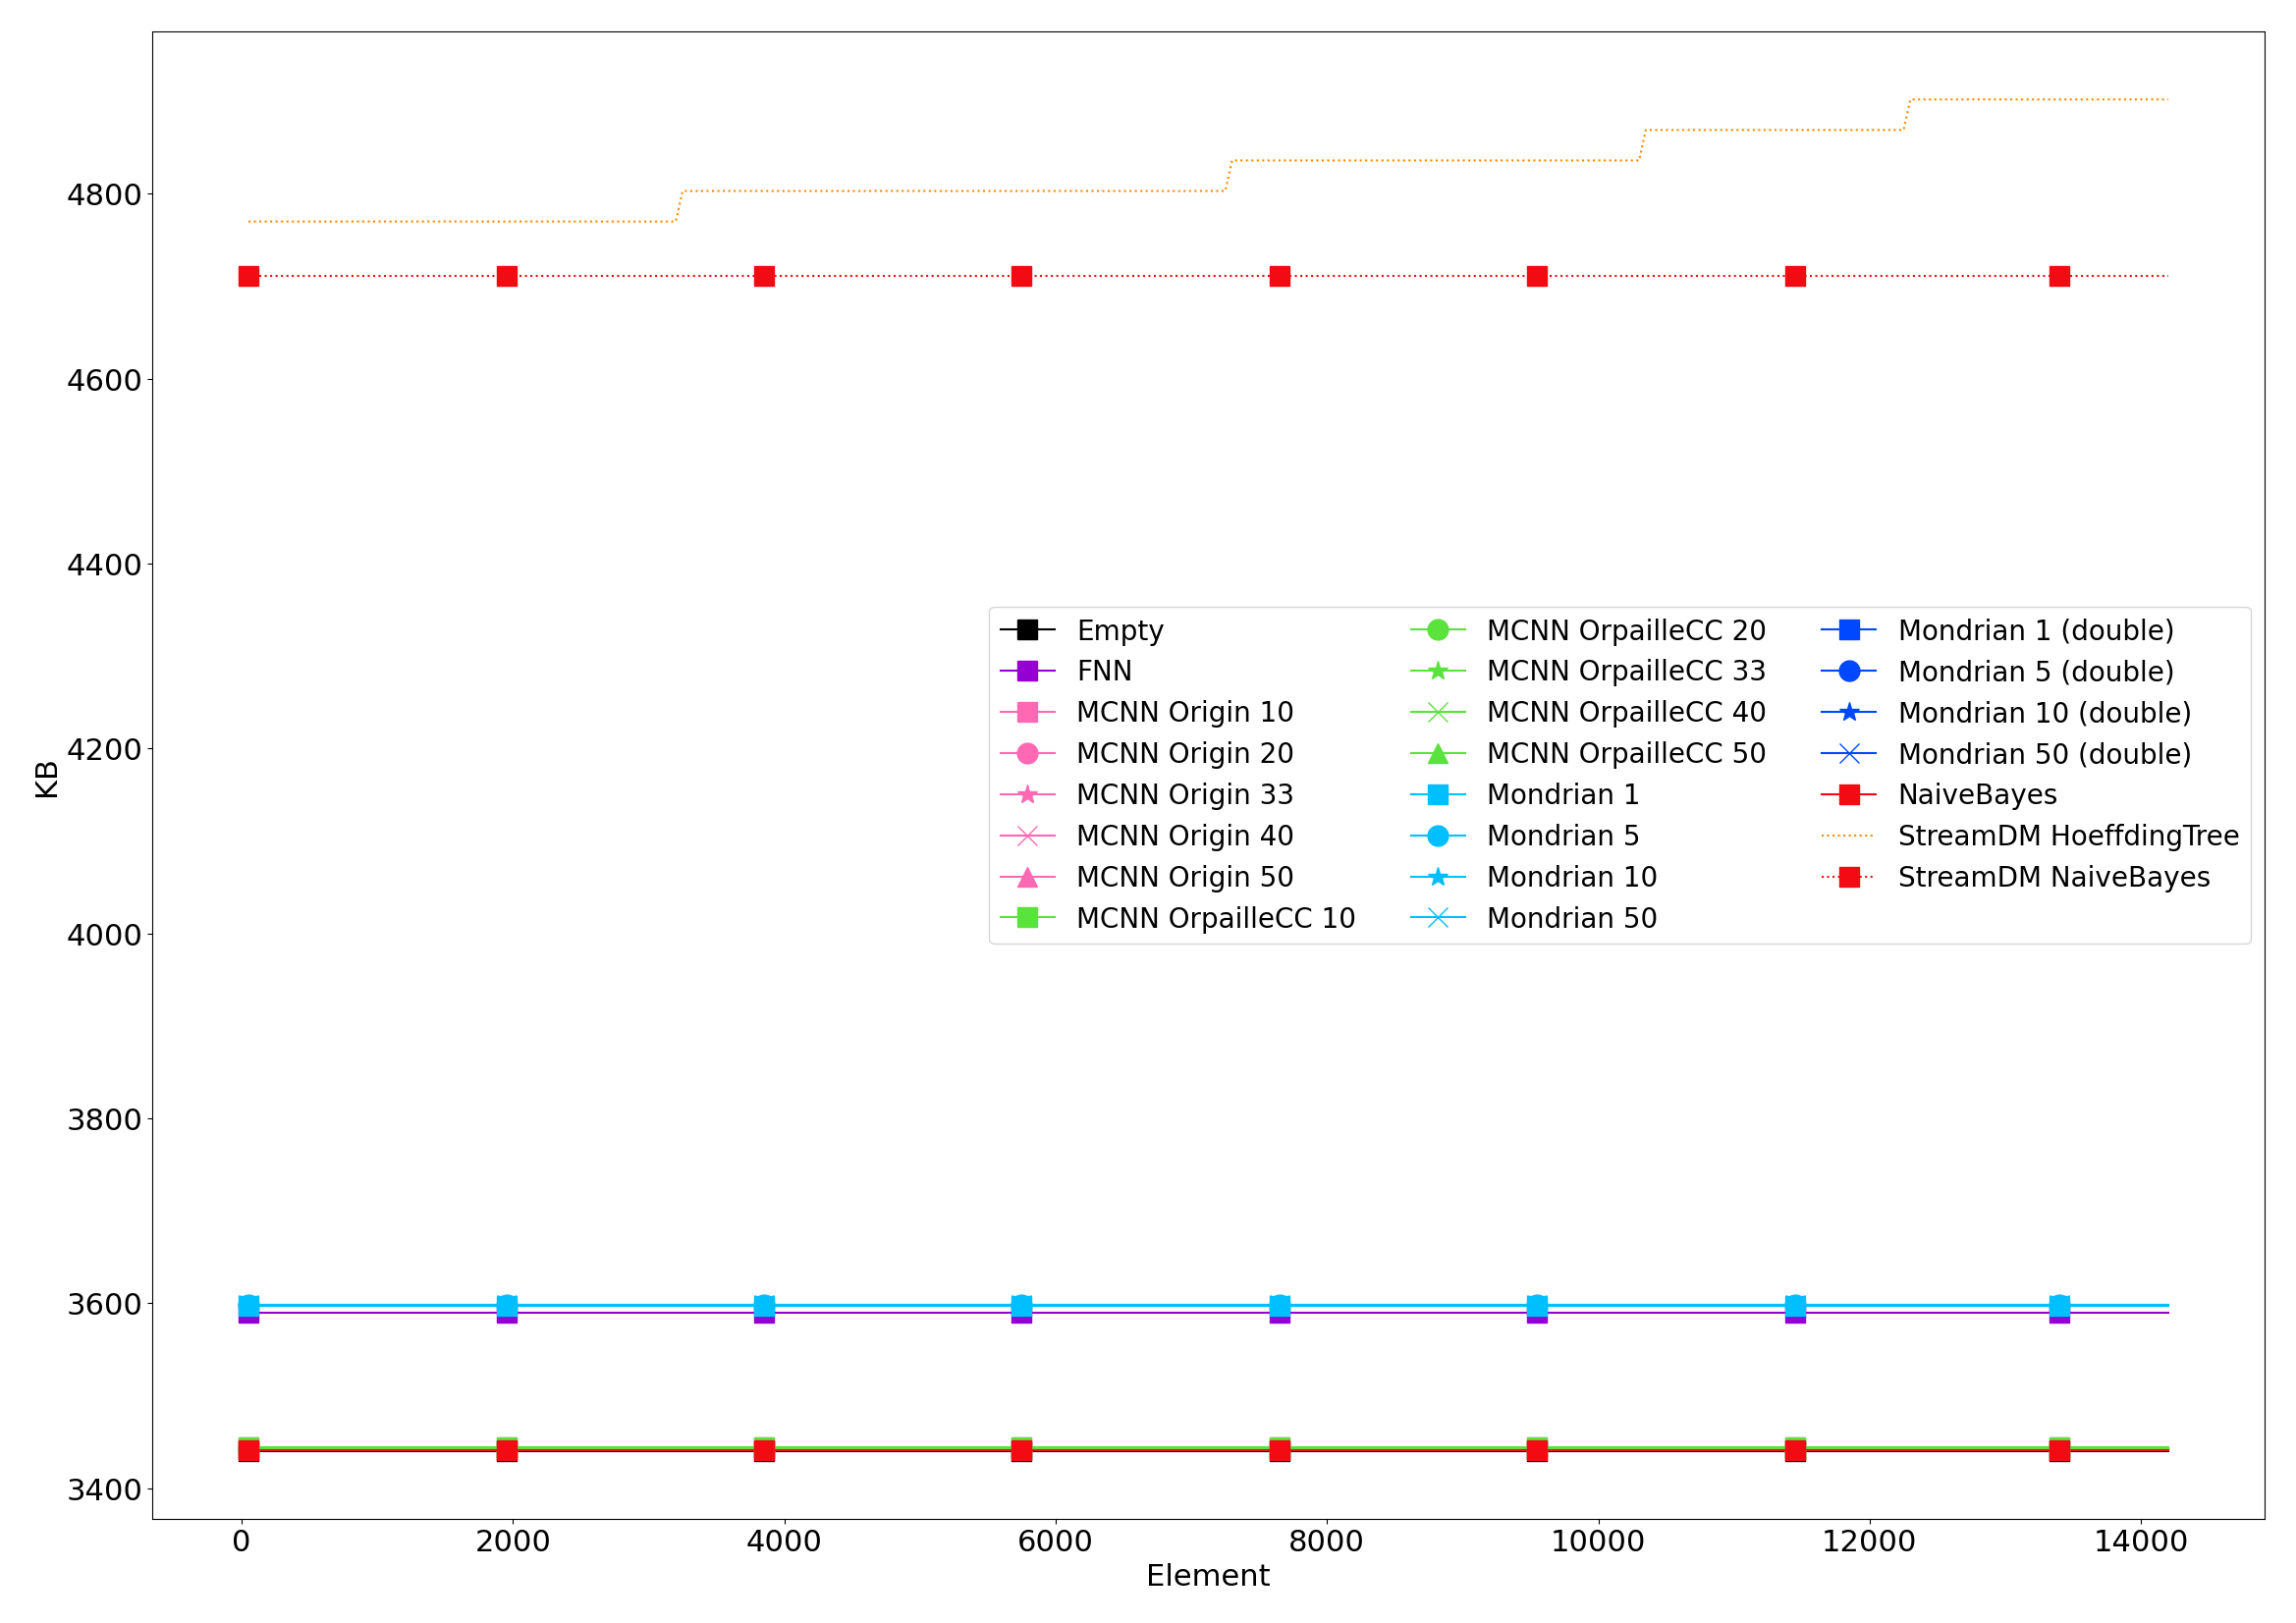
\includegraphics[width=\linewidth]{figures/results/banos_3_memory.png}
	\label{fig:memory}
	\caption{Memory used by the algorithms on the Banos dataset.}
\end{figure}


%\subsection{Micro-Cluster Nearest Neighbor tuning}
%Figure~\ref{fig:mcnn-tuning-error} show the impact of the error threshold on different number of cluster.
%\begin{figure}[H]
     %\begin{subfigure}[b]{0.49\textwidth}
         %\centering
		 %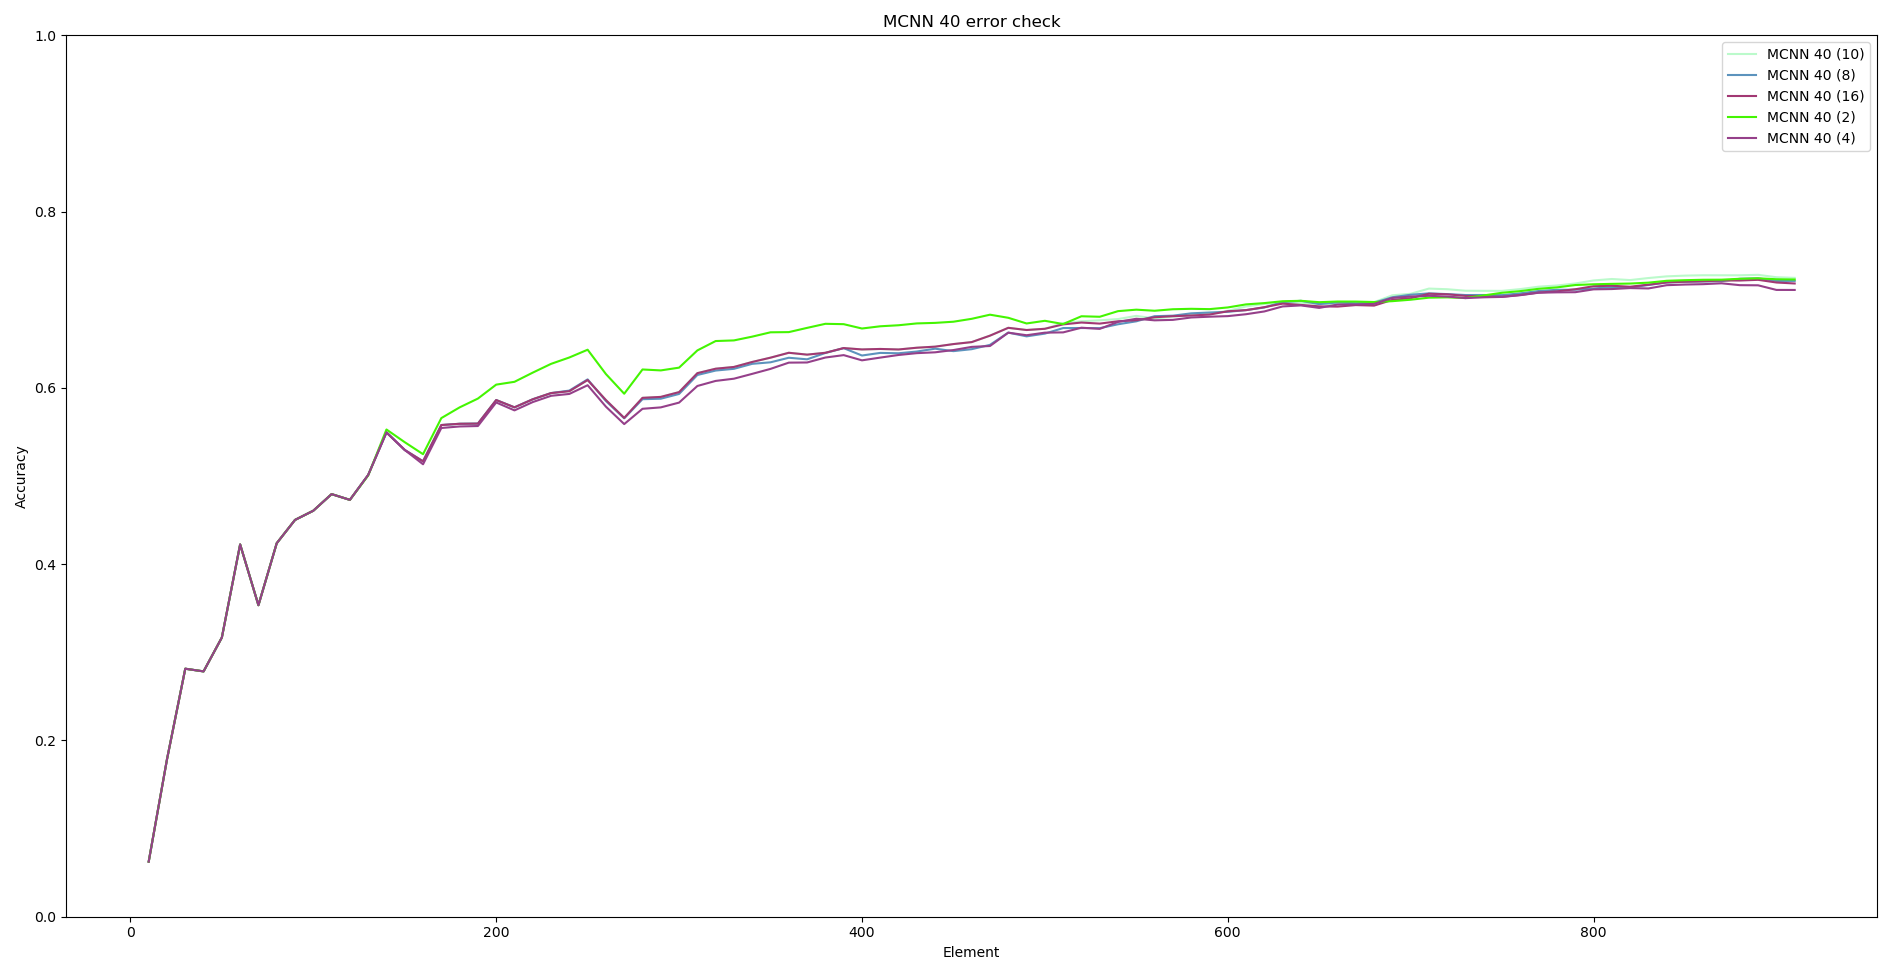
\includegraphics[width=\linewidth]{figures/Banos_S1_shuf_MCNN_40_error_check.png}
         %\caption{40 clusters}
     %\end{subfigure}
     %\begin{subfigure}[b]{0.49\textwidth}
         %\centering
		 %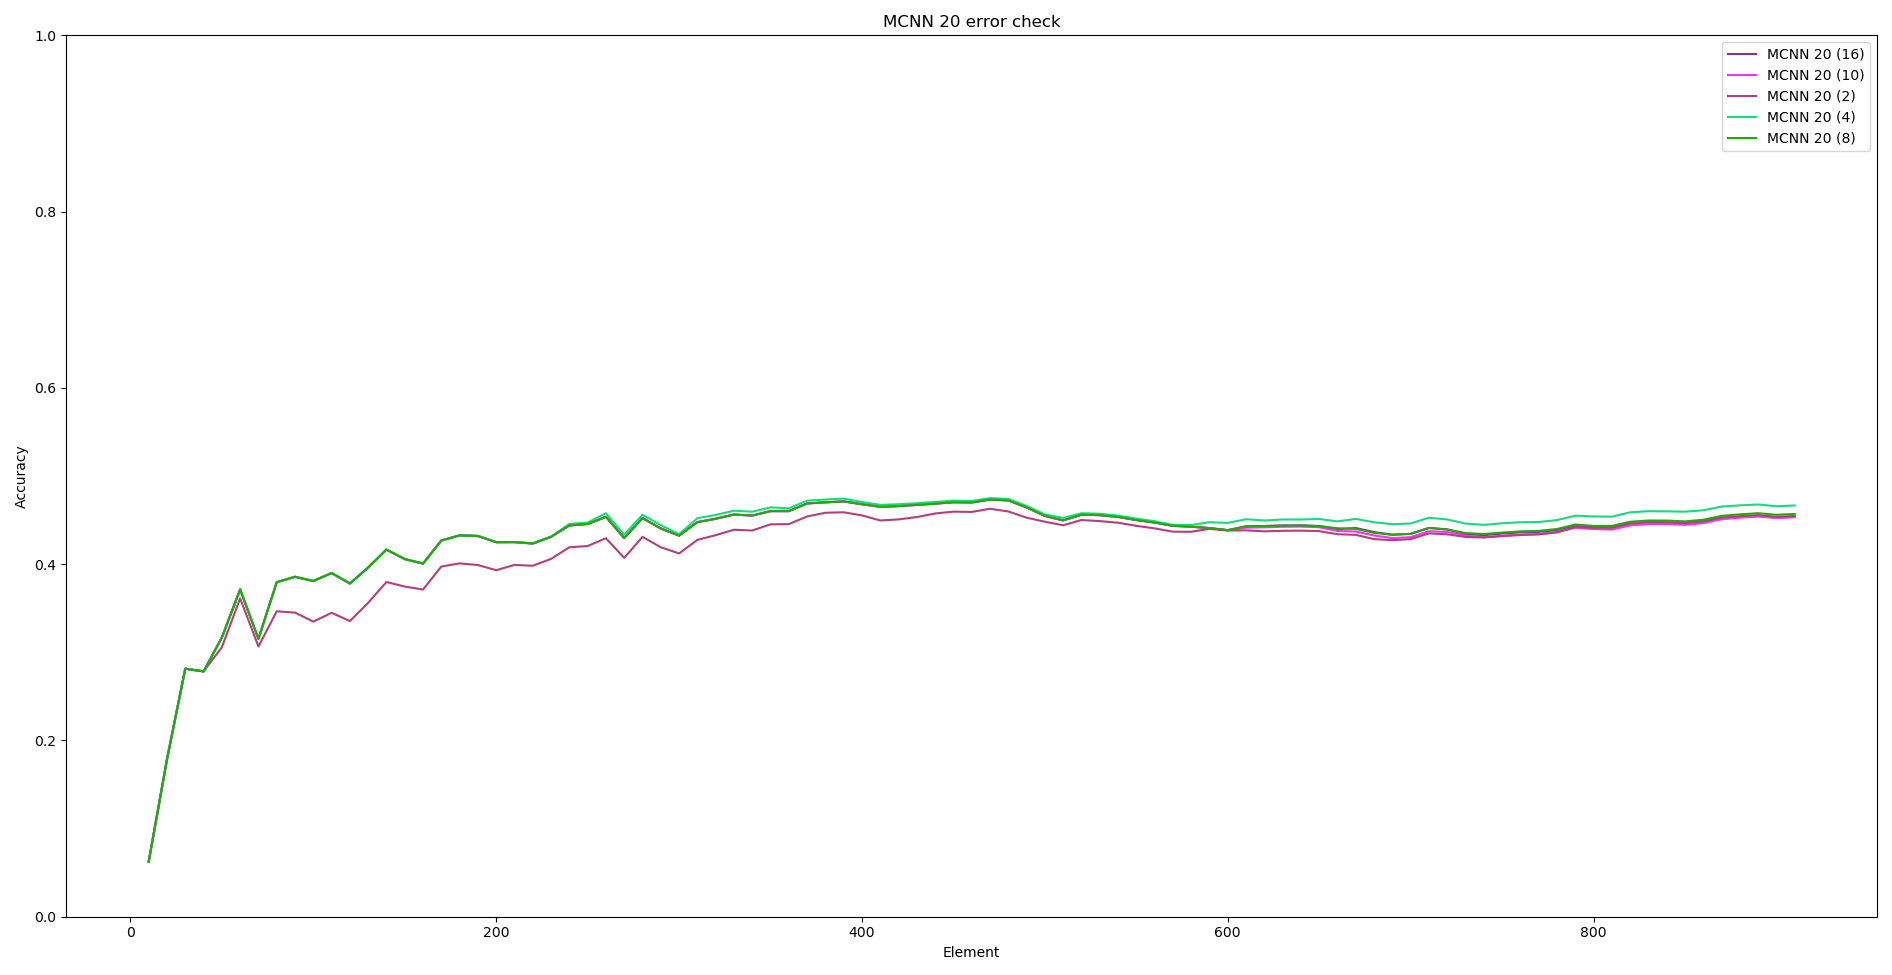
\includegraphics[width=\linewidth]{figures/Banos_S1_shuf_MCNN_20_error_check.png}
         %\caption{20 clusters}
     %\end{subfigure}
     %\begin{subfigure}[b]{0.49\textwidth}
         %\centering
		 %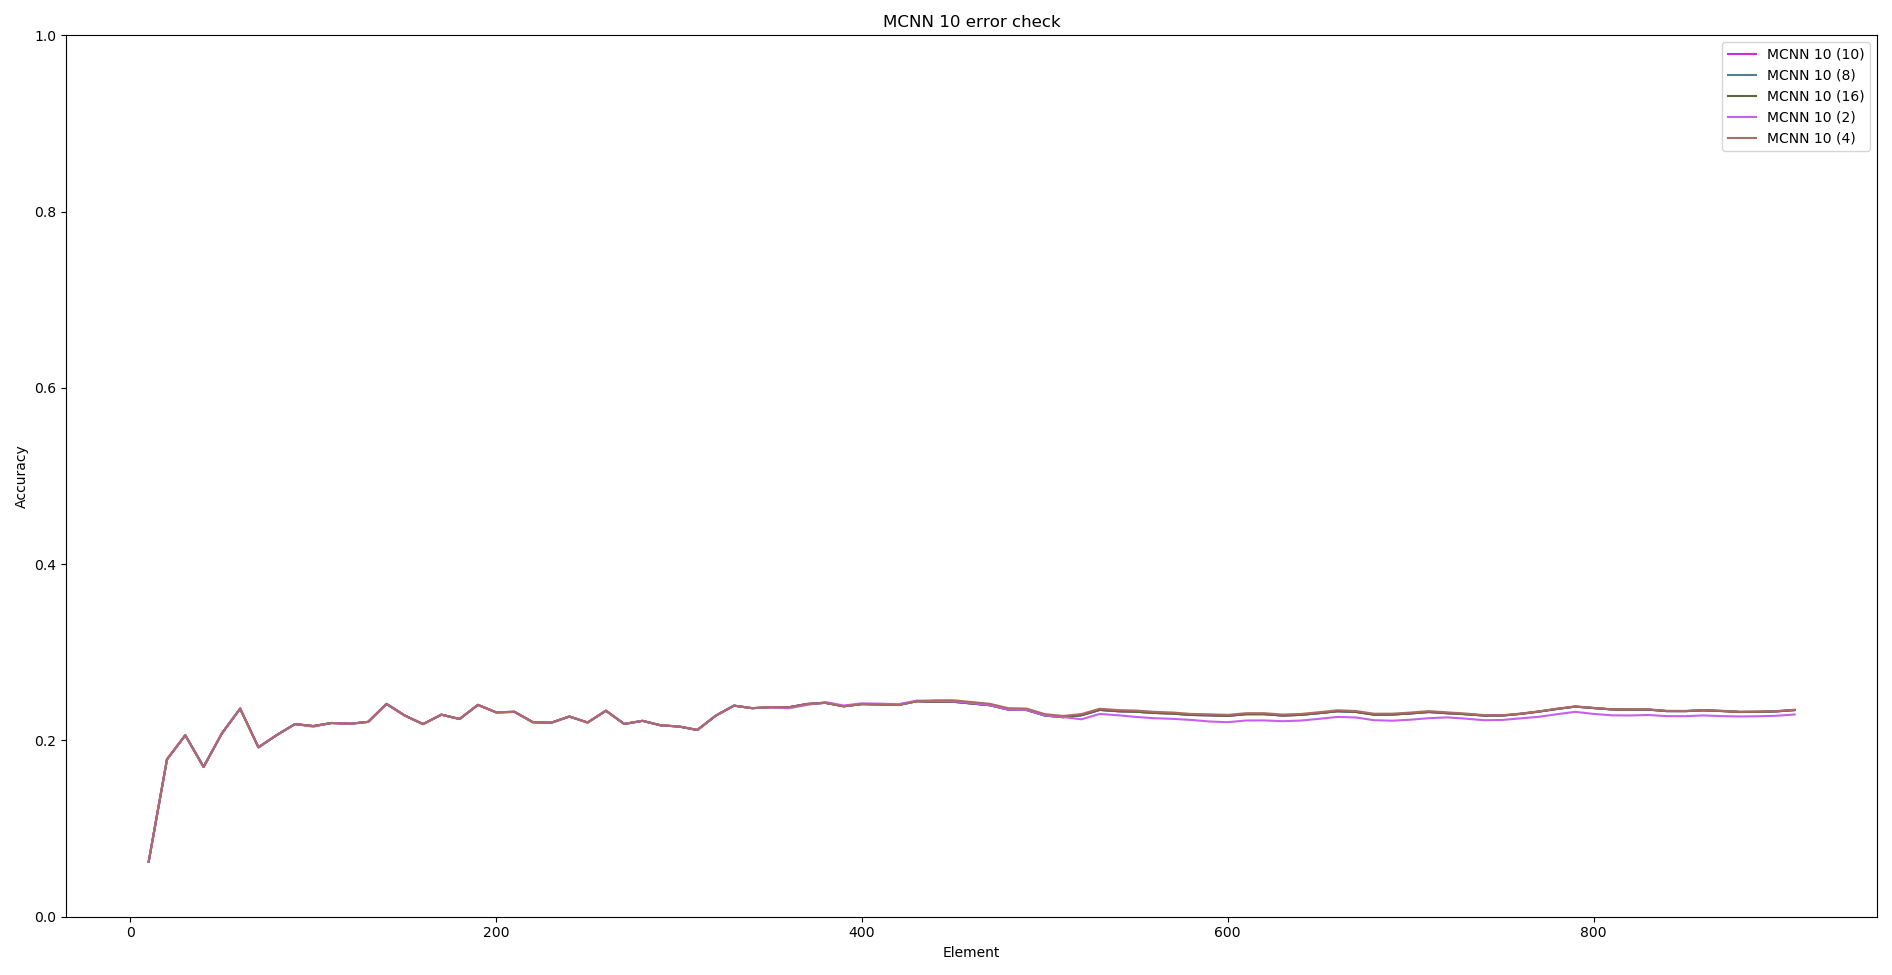
\includegraphics[width=\linewidth]{figures/Banos_S1_shuf_MCNN_10_error_check.png}
         %\caption{10 clusters}
     %\end{subfigure}
	%\caption{MCNN error}
	%\label{fig:mcnn-tuning-error}
%\end{figure}

%\subsection{Mondrian Tuning}
%Figure~\ref{fig:mondrian-tuning} show the impact of the Mondrian parameters on
%the accuracy. Occasionnaly, dashed lines are used to emphasis the minimum and
%the maximum.
%\begin{figure}
     %\centering
     %\begin{subfigure}[b]{0.49\textwidth}
         %\centering
         %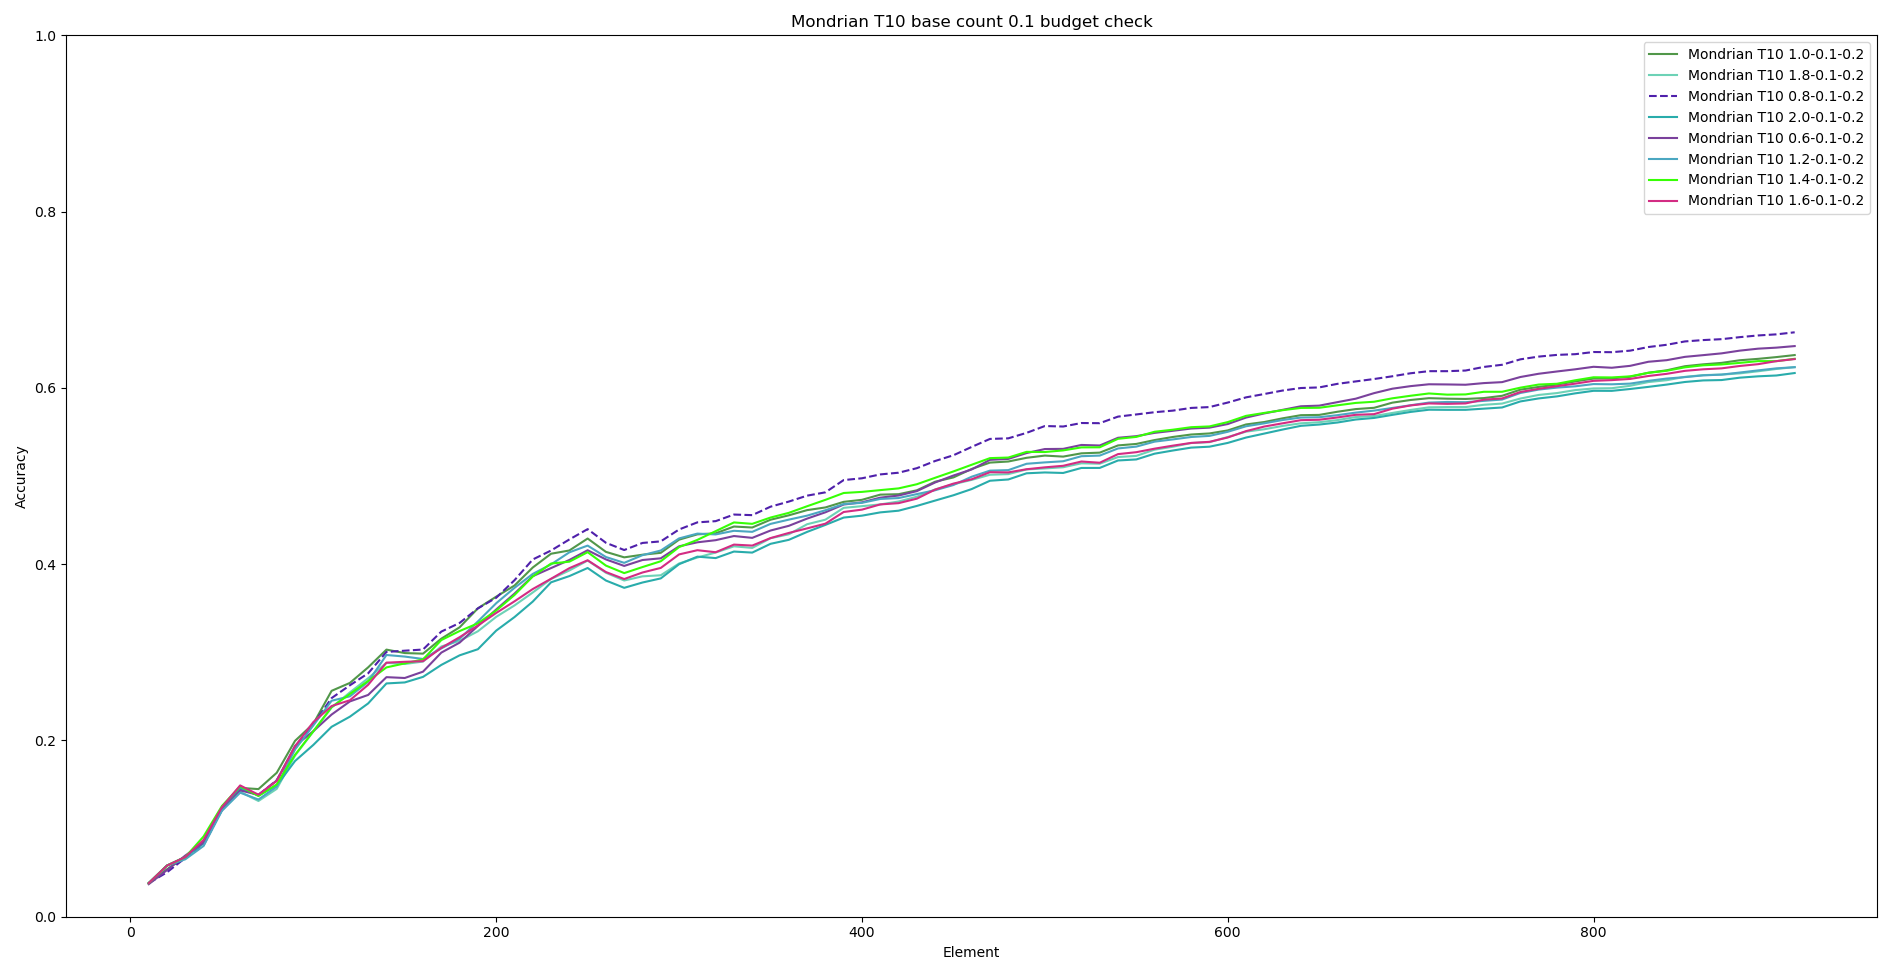
\includegraphics[width=\textwidth]{figures/Banos_S1_shuf_Mondrian_T10_bc_0.1_budget_check.png}
         %\caption{Impact of the $budget$ with 10 trees, a base count of $0.1$, and discount factor of $0.2$.}
     %\end{subfigure}
     %\hfill
     %\begin{subfigure}[b]{0.49\textwidth}
         %\centering
         %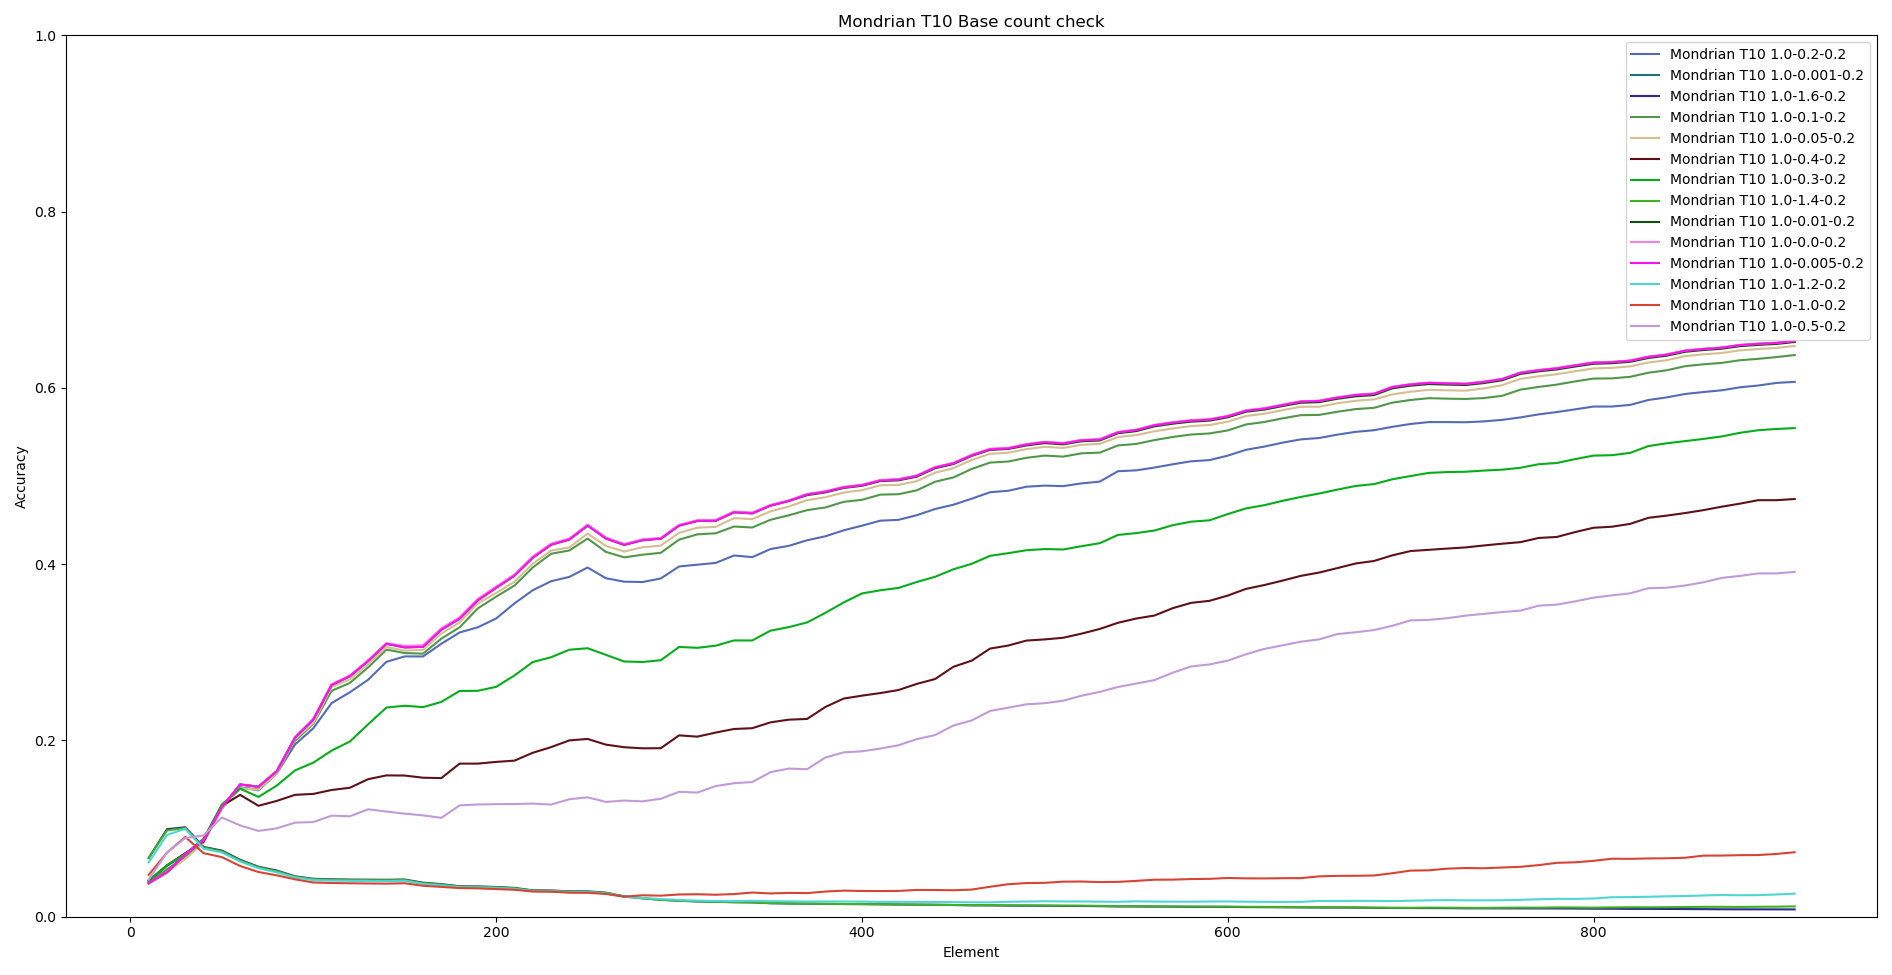
\includegraphics[width=\textwidth]{figures/Banos_S1_shuf_Mondrian_T10_check.png}
         %\caption{Impact of the base count with 10 trees, a budget of $1.0$, and a discount factor of $0.2$.}
     %\end{subfigure}
     %\hfill
     %\begin{subfigure}[b]{0.49\textwidth}
         %\centering
         %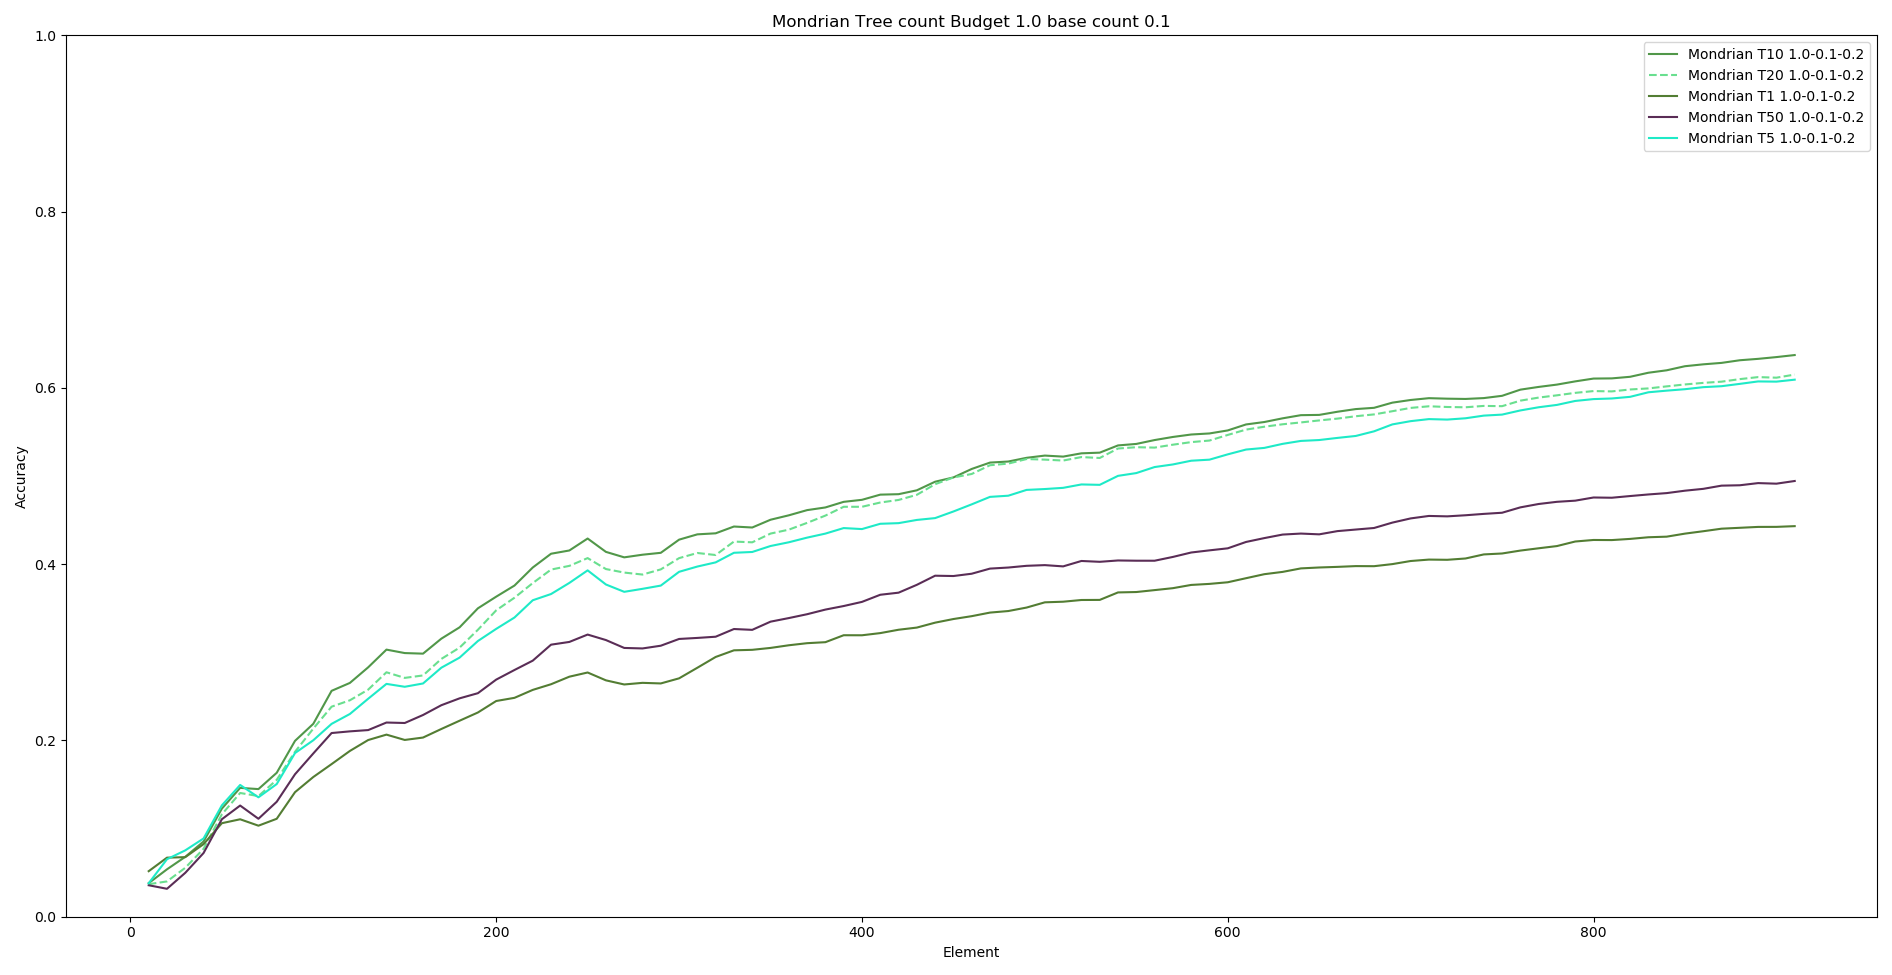
\includegraphics[width=\textwidth]{figures/Banos_S1_shuf_Mondrian_tree_count_fixed_other_bc0.1.png}
         %\caption{Impact of the tree count with a budget of $1.0$, a base count of $0.1$, and a discount factor of $0.2$.}
     %\end{subfigure}
     %\begin{subfigure}[b]{0.49\textwidth}
         %\centering
         %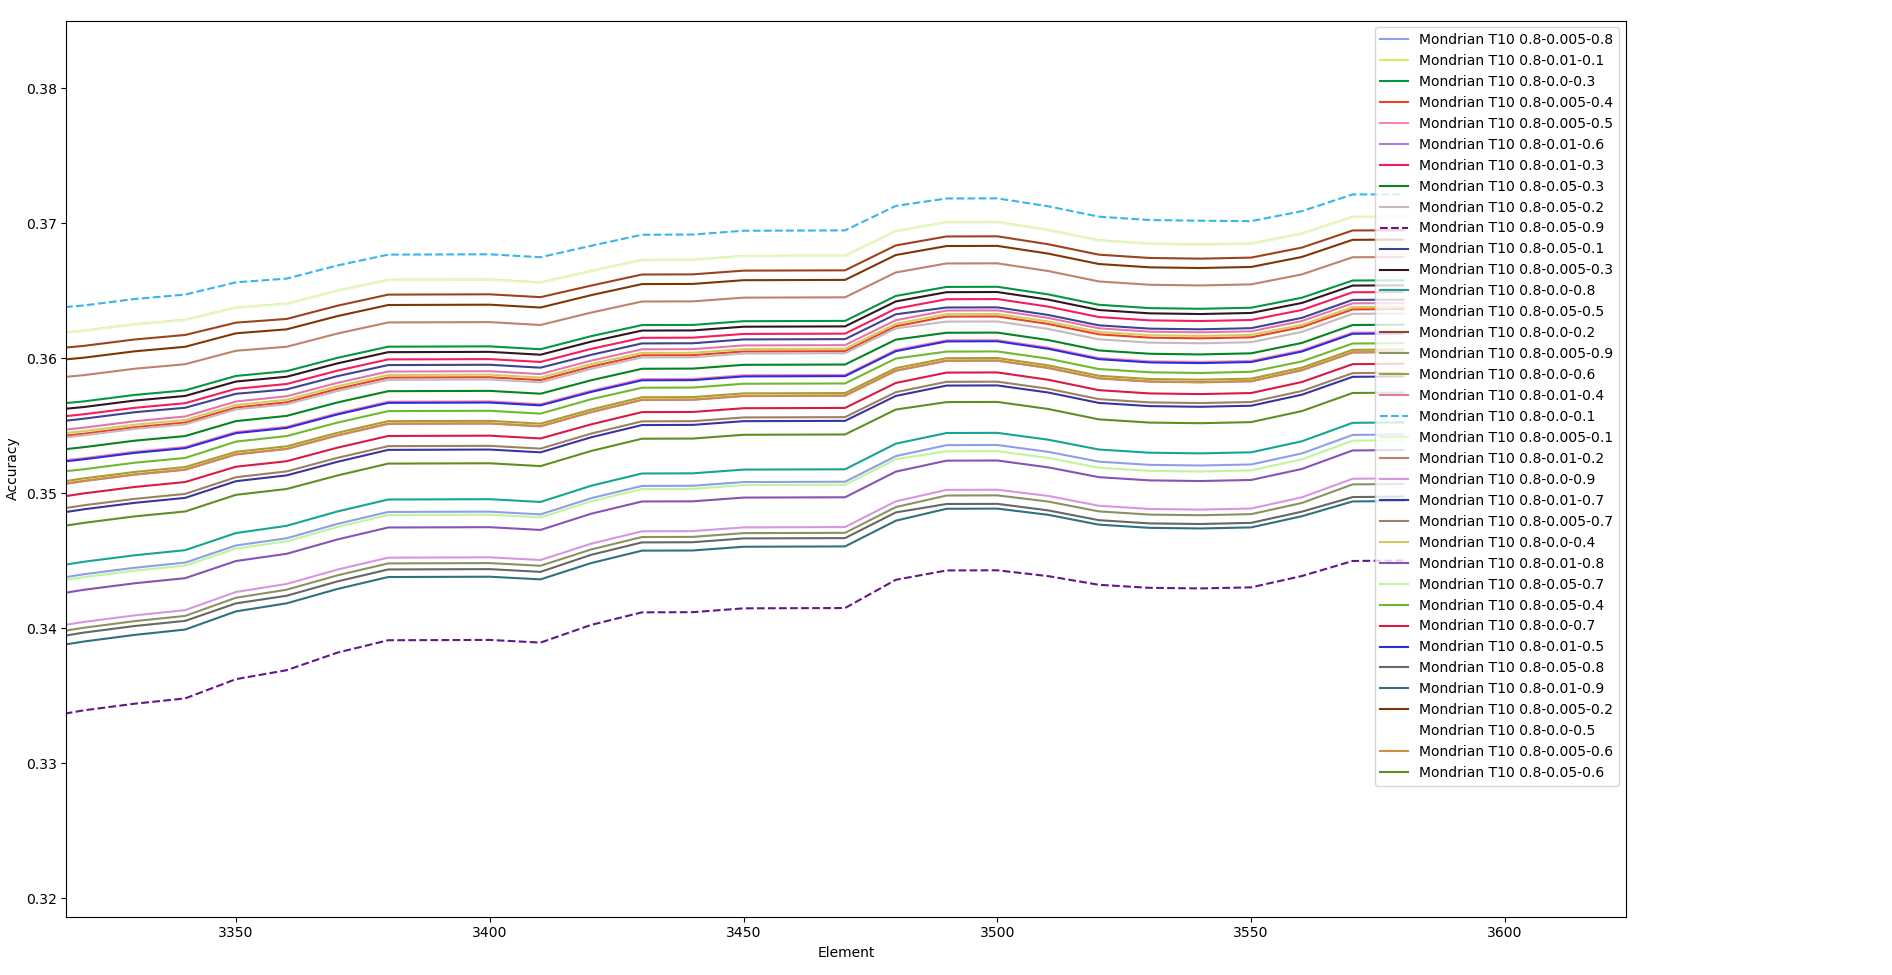
\includegraphics[width=\textwidth]{figures/Banos_S1_disount_check.png}
         %\caption{Impact of the discount factor with 10 trees, a budget of $1.0$, and a base count of $0.1$.}
     %\end{subfigure}
        %\caption{Mondrian tuning results.}
        %\label{fig:mondrian-tuning}
%\end{figure}


